%%%%%%%%%%%%%%%%%%%%%%%%%%%%%%%%%%%%%%%%%%%%%%%%%%%%%%%%%%%%
%%% LIVECOMS ARTICLE TEMPLATE FOR BEST PRACTICES GUIDE
%%% ADAPTED FROM ELIFE ARTICLE TEMPLATE (8/10/2017)
%%%%%%%%%%%%%%%%%%%%%%%%%%%%%%%%%%%%%%%%%%%%%%%%%%%%%%%%%%%%
%%% PREAMBLE
\documentclass[9pt,tutorial]{livecoms}
% Use the 'onehalfspacing' option for 1.5 line spacing
% Use the 'doublespacing' option for 2.0 line spacing
% Use the 'lineno' option for adding line numbers.
% Use the "ASAPversion' option following article acceptance to add the DOI and relevant dates to the document footer.
% Use the 'pubversion' option for adding the citation and publication information to the document footer, when the LiveCoMS issue is finalized.
% The 'bestpractices' option for indicates that this is a best practices guide.
% Omit the bestpractices option to remove the marking as a LiveCoMS paper.
% Please note that these options may affect formatting.

% NOTES
% when importing references from EndNote, remove the type = {Journal Article}. It messes with the livecoms bibtex style somehow...
% Place a \@ between all-caps words and punctuation ("This is a sentence about GIST\@. This is ...")
% Place a protected space (~) between "Figure" and the reference. The same with tables.

\usepackage{lipsum} % Required to insert dummy text
\usepackage[version=4]{mhchem}
\usepackage{siunitx}
\usepackage{float}
\usepackage{placeins}
\DeclareSIUnit\Molar{M}
\DeclareSIUnit\calorie{cal}
\DeclareSIUnit\kcalPerMolASqr{\kilo\calorie\per\mole\per\angstrom\squared}
%\DeclareSIUnit{\Molar}{M}
\DeclareSIUnit\angstrom{\text{\AA}}
%\DeclareSIPrefix\micro{\text{\textmu}}{0}
\sisetup{
	%math-rm=\mathsf,
	text-rm=\sffamily
}

\usepackage[italic,LGRgreek]{mathastext}
\graphicspath{{figures/}}

\usepackage{caption}
\usepackage{subcaption}
\usepackage{listings}
\usepackage{upquote}
\usepackage{tabularx}

%%%%%%%%%%%%%%%%%%%%%%%%%%%%%%%%%%%%%%%%%%%%%%%%%%%%%%%%%%%%
%%% IMPORTANT USER CONFIGURATION
%%%%%%%%%%%%%%%%%%%%%%%%%%%%%%%%%%%%%%%%%%%%%%%%%%%%%%%%%%%%

\newcommand{\versionnumber}{1.0}  % you should update the minor version number in preprints and major version number of submissions.
\newcommand{\githubrepository}{\url{https://github.com/liedllab/gist-tutorial}}  %this should be the main github repository for this article

%%%%%%%%%%%%%%%%%%%%%%%%%%%%%%%%%%%%%%%%%%%%%%%%%%%%%%%%%%%%
%%% ARTICLE SETUP
%%%%%%%%%%%%%%%%%%%%%%%%%%%%%%%%%%%%%%%%%%%%%%%%%%%%%%%%%%%%
\title{Tutorial: Quantifying Spatially Resolved Hydration Thermodynamics Using Grid Inhomogeneous Solvation Theory [Article v\versionnumber]}

\author[1\authfn{1}]{Valentin J Hoerschinger}
\author[1\authfn{1}]{Franz Waibl}
\author[2]{Vjay Molino}
\author[2]{Helmut Carter}
\author[1]{Monica L Fern{\'a}ndez-Quintero}
\author[2]{Steven Ramsey}
\author[4]{Daniel R Roe}
\author[1*]{Klaus R Liedl}
\author[3*]{Michael K Gilson}
\author[2*]{Tom Kurtzman}

\affil[1]{Department of General, Inorganic and Theoretical Chemistry, University of Innsbruck, Austria}
\affil[2]{Department of Chemistry, Lehman College, The City University of New York, Bronx, New York, USA}
\affil[3]{Skaggs School of Pharmacy and Pharmaceutical Sciences, University of California, San Diego, USA}
\affil[4]{Laboratory of Computational Biology, National Heart, Lung, and Blood Institute, National Institutes of Health, Bethesda, Maryland, USA}

\corr{klaus.liedl@uibk.ac.at}{KRL}
\corr{mgilson@health.ucsd.edu}{MKG}
\corr{thomas.kurtzman@lehman.cuny.edu}{TK}
%TODO Vjays ORCID is missing
\orcid{Valentin J Hoerschinger}{0000-0002-4469-3238}
\orcid{Franz Waibl}{0000-0003-0527-0803}
\orcid{Vjay Molino}{}
\orcid{Helmut Carter}{0000-0003-0273-4107}
\orcid{Monica L Fern{\'a}ndez-Quintero}{0000-0002-6811-6283}
\orcid{Steven Ramsey}{0000-0001-7441-3228}
\orcid{Daniel R Roe}{0000-0002-5834-2447}
\orcid{Klaus R Liedl}{0000-0002-0985-2299}
\orcid{Michael K Gilson}{0000-0002-3375-1738}
\orcid{Tom Kurtzman}{0000-0003-0900-772X}

\contrib[\authfn{1}]{These authors contributed equally to this work}


\blurb{This LiveCoMS document is maintained online on GitHub at \githubrepository; to provide feedback, suggestions, or help improve it, please visit the GitHub repository and participate via the issue tracker.}

%%%%%%%%%%%%%%%%%%%%%%%%%%%%%%%%%%%%%%%%%%%%%%%%%%%%%%%%%%%%
%%% PUBLICATION INFORMATION
%%% Fill out these parameters when available
%%% These are used when the "pubversion" option is invoked
%%%%%%%%%%%%%%%%%%%%%%%%%%%%%%%%%%%%%%%%%%%%%%%%%%%%%%%%%%%%
\pubDOI{10.XXXX/YYYYYYY}
\pubvolume{<volume>}
\pubissue{<issue>}
\pubyear{<year>}
\articlenum{<number>}
\datereceived{Day Month Year}
\dateaccepted{Day Month Year}


%%% Shortcuts and macros
\newcommand{\dgsolv}{\Delta G_\textup{solv}}
\newcommand{\software}{\texttt}
\newcommand{\code}{\texttt}
\newcommand{\todo}{\textcolor{red}}
\newcommand\inlinecode{\texttt}

% The \neq command looks messy by default. Replace it by our own makeshift version.
\renewcommand{\neq}{\setbox0\hbox{=}\rlap{\hbox to \wd0{\hss /\hss}}\box0}

\lstset{
	basicstyle=\ttfamily\footnotesize,
	inputencoding=utf8,
	extendedchars=true,
	literate={Å}{{\AA}}1,
	backgroundcolor = \color[rgb]{0.9, 0.9, 0.9},
	showstringspaces=false,
	columns=fullflexible,
}
\lstdefinestyle{code}{}
\lstdefinestyle{cpptraj}{title={\centering cpptraj}}
\lstdefinestyle{bash}{title={\centering Command-line}}
\lstdefinestyle{amber-in}{title={\centering Amber input}}
\lstdefinestyle{pymol}{title={\centering Pymol}}
\lstdefinestyle{python}{
	title={\centering Python},
	language=Python,
	stringstyle=\color[rgb]{1.0, 0, 0},
	commentstyle=\color[rgb]{0, 0, 0.6}
}
\lstset{style=code}


% TODO: delete for final build
\usepackage{pdfcomment}

%%%%%%%%%%%%%%%%%%%%%%%%%%%%%%%%%%%%%%%%%%%%%%%%%%%%%%%%%%%%
%%% ARTICLE START
%%%%%%%%%%%%%%%%%%%%%%%%%%%%%%%%%%%%%%%%%%%%%%%%%%%%%%%%%%%%

\begin{document}

\begin{frontmatter}
\maketitle

\begin{abstract}
Grid inhomogeneous solvation theory (GIST) is a method to compute the free energy of solvation of a solute molecule on a 3-dimensional grid based on sampling from molecular dynamics (MD) simulations.
The high spatial resolution of the GIST output, as well as the decomposition into energy and entropy contributions, allow for highly detailed analyses of solvation around both proteins and small molecules contexts. 
However, this versatility also comes with a significant entry barrier for new users.

In this tutorial, we aim to guide the reader through the most common steps involved in a GIST analysis using the streptavidin-biotin complex as an demonstrative system. Towards this, Jupyter notebooks and Python packages are provided to simplify the analysis.
Furthermore, we discuss the theory of GIST with a focus on practical aspects.
We highlight potential pitfalls and show how to avoid technical difficulties.
For this tutorial, familiarity with molecular dynamics simulations as well as the AmberTools package \cite{Case2023-ambertools} is assumed. 

%This particular document provides a skeleton illustrating key sections for a Tutorial document.
%Please see the sample \texttt{sample-document.tex} in \url{github.com/livecomsjournal/article_templates/templates} for additional information on and examples of using the LiveCoMS LaTeX class.
%Here we also assume familiarity with LaTeX and knowledge of how to include figures, tables, etc.; if you want examples, see the sample just referenced.
%
%In your work, in this particular slot, please provide an abstract of no more than 250 words.
%Your abstract should explain the main contributions of your article, and should not contain any material that is not included in the main text.
%Please note that your abstract, plus the authorship material following it, must not extend beyond the title page or modifications to the LaTeX class will likely be needed.
\end{abstract}

\end{frontmatter}

\begin{figure}[H]
	\centering
	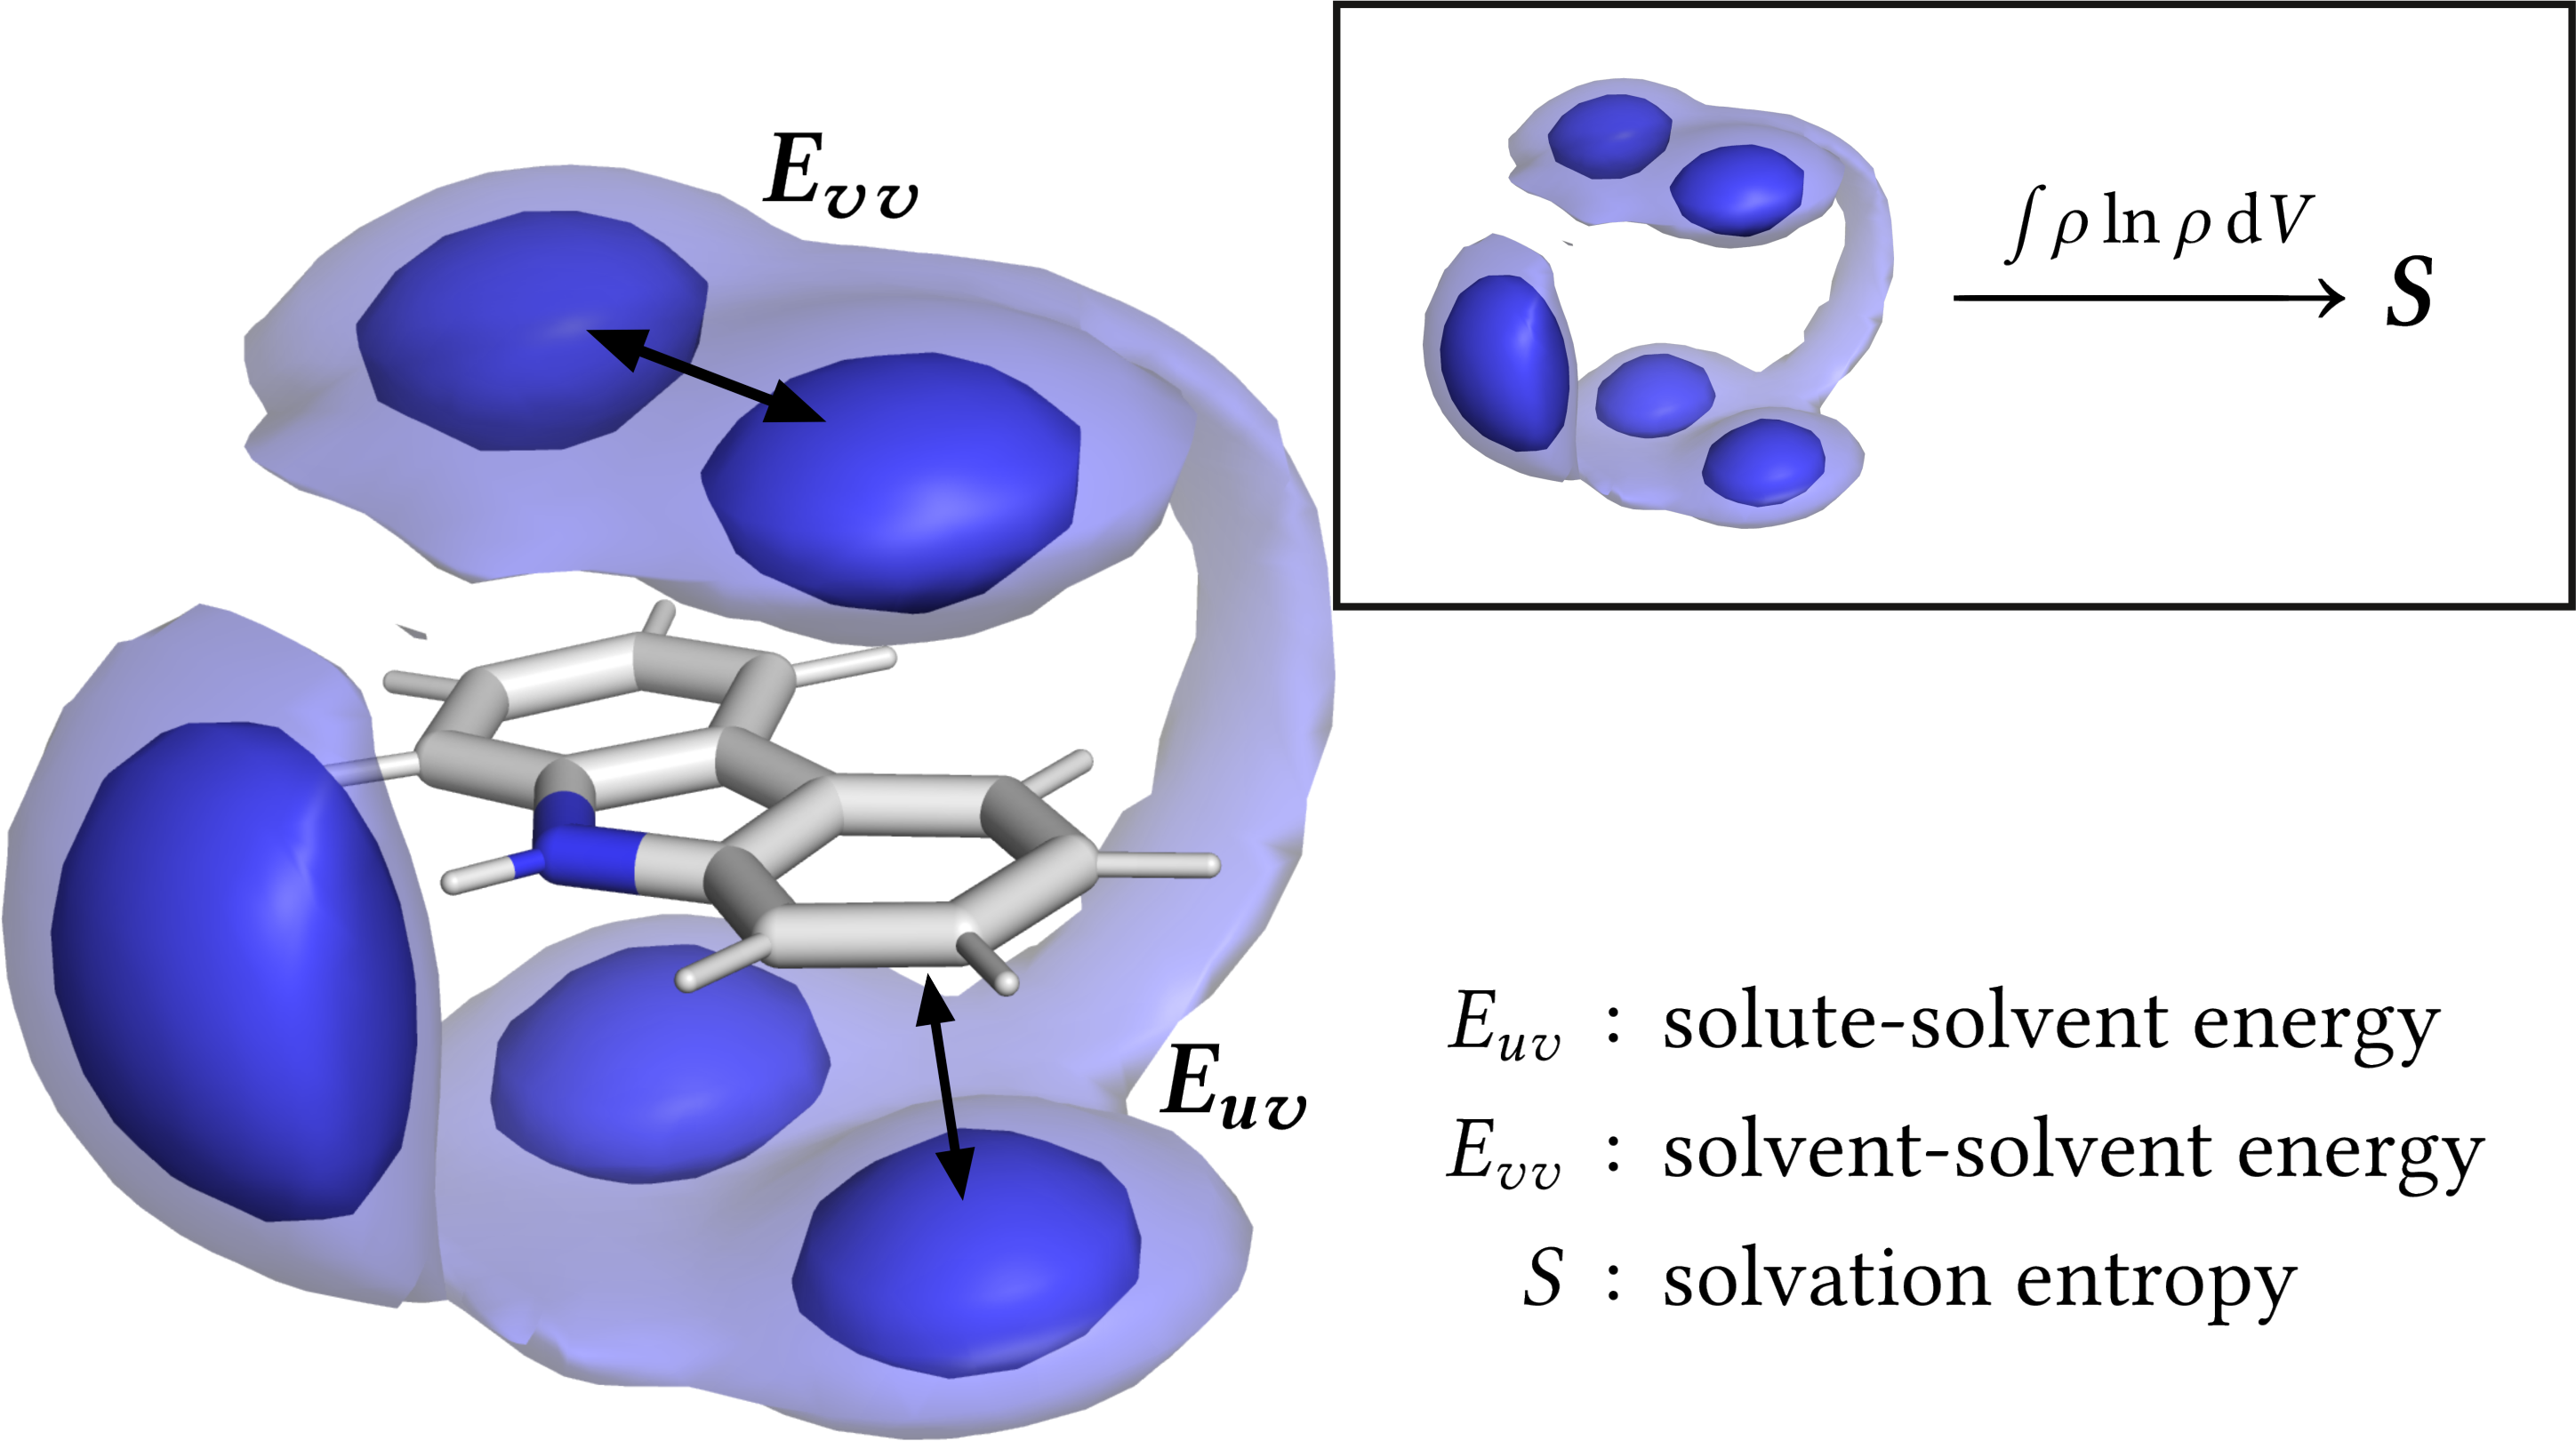
\includegraphics[width=\linewidth]{figures/carbazole-figure.png}
	\caption{Schematic showing regions of high water density around a carbazole solute molecule. Based on an MD simulation of solvent around the solute molecule, the energy is computed from the intermolecular interactions of a force field, while the entropy is approximated from the 6-dimensional orientational and solvational solvent distribution $\rho$ around the solute molecule. Note that while this depiction focuses on regions of high solvent density, regions with lower density can also contain meaningful contributions to the overall energy and entropy.}
	\label{fig:carbazole}
\end{figure}
\section{Introduction}
Solvation thermodynamics govern many biological and chemical processes involving, e.g., aqueous solutions, hydrophobic effects, or partitioning between different environments.
Interactions with water are of special importance as many biological processes occur in an aqueous environment \cite{Privalov2017-water-review}.
The free energy of solvation is defined as the reversible work needed to insert a solute molecule into the solvent from gas phase \cite{ben-naim-book}.
It is directly linked to the solubility of gases and drives many real-world effects such as hydrophobicity, ligand binding, and protein folding.

Grid inhomogeneous solvation theory (GIST) \cite{Nguyen2012} is a method to compute the free energy of solvation, with applications in the context of drug design and biophysical property description.
It computes the solvent density from an MD trajectory and estimates localized entropic and enthalpic contributions on a grid around the solute molecule.
Since these contributions are spatially resolved, GIST improves interpretability and offers more detailed insights into the solvation of the investigated solute.
A schematic of this is shown in Figure~\ref{fig:carbazole}.  
The entropy is computed from orientational and translational distributions of the solvent around the solute molecule, in a first-order approximation. 
The calculation of higher-order entropy terms is computationally demanding but was realized in recent works \cite{Nguyen2016-gist-second-order, Waibl2021-gist-salt}.
It has been found that solvation free energies of small molecule solutes can be computed at high accuracy using linear scaling factors for the higher-order terms, such as $\Delta S = 0.6\, \Delta S^\text{1st-order}$ for water \cite{Chen2021,Waibl2022-gist-solvents}.
Since its initial development, GIST has been used to describe the thermodynamics of water displacement in protein binding pockets \cite{Nguyen2016-gist-second-order,Ramsey2016,Balius2017-gist-ligand-discovery,Hufner-Wulsdorf2020-gist-drug-design}.
It has been used for a large-scale investigation of the hydration properties of proteins found in SARS-CoV-2 \cite{Olson2020-covid-gist}.
Furthermore, recent works used GIST to describe biophysical properties of serine proteases \cite{Kraml2019-gigist}, macrocycles \cite{Kamenik2020-gist-macrocycles}, or antibody fragements \cite{Waibl2021-gist-antibodies}.

GIST has been implemented on the GPU, substantially improving its performance for large grids \cite{Kraml2019-gigist}.
Furthermore, an implementation based on the particle mesh Ewald (PME) \cite{Darden1993-pme} method improves both the efficiency and the agreement with popular molecular dynamics engines \cite{Chen2021}. 
Yet further changes allow the inclusion of other rigid solvents than water \cite{Kraml2020,Waibl2022-gist-solvents} or the use of salt-water mixtures as solvents \cite{Waibl2021-gist-salt}.

In this tutorial, we aim to give the reader an introduction to GIST and its application to calculate solution thermodynamics properties of interest. 
While previous publications \cite{Ramsey2016} and tutorials \cite{amber_tut_gist} treated how to setup and run GIST calculations in detail, the post-processing was often treated in less detail. 
While building on these tutorials, we provide an updated guide to calculating solvation properties using GIST to address recent improvements.
Furthermore, we aim to establish best practices for the analysis and interpretation of GIST calculations.

\subsection{Comparison to other methods}
A wide range of methods have been devised to compute the free energy of hydration.
Data-driven methods include QSPR and UNIFAC \cite{Borhani2019-qspr,Fredenslund1975-unifac}.
Polarizable continuum models (PCMs) \cite{Miertus1981-pcm,Klamt1993-cosmo} treat the solvent as a homogeneous phase that reacts to the electrostatic potential of the solute molecule \cite{Mennucci2010-pcm}.
%Molecular mechanics based approaches describe the underlying PES through empirically fit force-fields, which reduce the computational demand of these calculations tremendously.
%This allows for the treatment of large biological systems such as proteins in aqueous solution.
Methods such as MM/PBSA or MM/GBSA \cite{Sitkoff1994-pbsa,Kollman2000-mmpbsa} combine an implicit treatment of solvent electrostatics with structural sampling of the solute molecule.
They can quickly provide results for a large number of structures \cite{Genheden2015-mmpbsa-review}.\\
On the other hand, explicit solvation methods model the solvent using individual molecules.
They are generally more accurate than implicit methods, but require a statistical sampling of the solvent conformations \cite{Liu2016-md-solubility,Swails2014-cphmd}.
Molecular dynamics (MD) simulations provide an accurate way of modeling solvent packing in confined areas \cite{Haider2016-water-on-surfaces} and general hydrophobic effects \cite{Pratt2016-hydrophobicity}.

The free energy of solvation can be calculated in a statistically rigorous way using alchemical methods \cite{Liu2016-md-solubility,Mobley2009-dgsolv,Mobley2014-freesolv} such as free energy perturbation (FEP) \cite{Zwanzig1954-reweighting} or thermodynamic integration (TI) \cite{Kirkwood1935-ti}.
However, those methods are unable to provide a spatial interpretation of the results.
Furthermore, splitting the free energy into enthalpy and entropy contributions is challenging \cite{Peter2004-alchemical-entropy}.\\
Methods derived from statistical mechanics bridge this gap by providing three-dimensional resolution.
These methods most commonly are based on either the Ornstein–Zernike (OZ) equation, or \cite{Hansen2013-simple-liquids} inhomogeneous fluid solvation theory (IST) \cite{Lazaridis1998}.
The most important example of OZ-based methods is the reference interaction site model (RISM) \cite{Chandler1972-rism} as well as its extension to three dimensions (3D-RISM) \cite{Kovalenko1998-3drism}.
Those methods compute the atomic solvent distributions by self-consistently solving the OZ integral equation to predict solvation thermodynamics.

Methods based on IST use a molecular solvent distribution obtained from an MD simulation to compute the free energy of hydration from its enthalpic and entropic contributions, providing easier interpretability of the resulting distributions.
Examples include grid inhomogeneous solvation theory (GIST) \cite{Nguyen2012,Ramsey2016}, WaterMap \cite{Young2007-watermap,Abel2008-watermap}, SSTMap \cite{Haider2018-sstmap}, STOW \cite{Li2012-stow} and Solvaware \cite{Huggins2016-solvaware}.
The main limitation of those methods is that the entropy is approximated through an infinite expansion in terms of the density distribution. 
Within GIST and other more recent methods, these entropy contributions are calulated via a k-nearest-neighbor (kNN) approach.  
Due to the high computational effort required to converge the higher order terms, the entropy expansion is usually truncated after the first or, sometimes, the second \cite{Nguyen2016-gist-second-order,Waibl2022-gist-solvents} term, thereby introducing an error.
While there are approximations available to deal with those problems, most noteworthy the mutual information expansion (MIE) and Maximum Information Spanning Tree (MIST) approaches, they are not currently implemented in GIST. 
Recent kNN implementations to calculate solvation entropy further improve phase space sampling by relabeling the solvent molecules in the simulation, treating the solvent molecules as distinguishable \cite{reinhard2007estimation,heinz2019computing,heinz2021permut,fogolari2021optimal}. For a recent review of kNN methods to calculate entropy in a molecular context, see \cite{fogolari2024k}.
Furthermore, IST does not consider the internal degrees of freedom of the solvent.
Therefore, IST-based approaches currently can only be used with sufficiently rigid solvents, although a recent paper provides the theory needed to generalize to flexible solvent molecules \cite{gilson2024freeenergy}.
Nevertheless, they have been applied on a wide variety of problems involving both small molecules and biological systems as solute molecules.\\
GIST is an implementation of IST on a three-dimensional grid. 
Unlike the related method WaterMap \cite{Abel2008-watermap,Young2007-watermap}, it provides solvation thermodynamics on an entire grid, rather than only high-density clusters in a binding pocket.
This implies a higher versatility, but also puts more responsibility on the user in terms of correct post-processing.
Since the density is computed from an explicit solvent MD simulation, GIST provides an accurate picture of solvation at an atomistic level, even for demanding systems such as drug binding sites in proteins.
While the need for MD simulations comes at a large computational cost, GIST is still more efficient than end-state approaches such as TI \cite{Kirkwood1935-ti} or FEP \cite{Zwanzig1954-reweighting}, with applications to large systems such as serine proteases \cite{Kraml2019-gigist} or antibody fragments \cite{Waibl2021-gist-antibodies}.
On the other hand, the first-order approximation means that the solvation entropy is less accurately described than in TI or FEP \cite{Chen2021,Waibl2021-gist-salt}. 
Similar to the self-consistent integral theories, GIST only considers a single solute conformation and  multiple computations of representative structures are necessary to describe ensemble properties. 

\subsection{Scope}
The purpose of this tutorial is to help users run GIST calculations and interpret the results.
The tutorial is structured around two examples: a GIST calculation for the small molecule biotin, and a GIST study of biotin-streptavidin binding. 
Whereas the biotin example gives an introduction to the basics of GIST calculations, the full biotin-streptavidin analysis showcases details and considerations commonly found in more advanced GIST studies.
We show how to interpret the three-dimensional contributions of solvation free energy in a binding pocket and around the ligand.
Additionally, we compute the binding contribution of the free energy of solvation, which requires accurate post-processing of the GIST outputs to avoid unfavorable summation of bias.
In total, we aim to provide a workflow that can be easily adapted to different systems, an introduction to the method and the theory behind it, and an overview of the different implementations of GIST.\\
Furthermore, we discuss several technical aspects of GIST studies, such as the normalization of voxel values. 
Additionally, we provide a Python library (\software{gisttools}) to unify the analysis of GIST data produced by various versions of GIST and make the post-processing of GIST results more accessible.
After completing this tutorial, we expect the reader to be able to run their own GIST study. 

%Tutorials should endeavor to cover the specific task at hand, and also highlight how the steps might need to be modified (or additional care might need to be taken at particular points) to handle more general cases.
%
%The scope of the tutorial, as well as the expected proficiencies / outcomes for researchers who complete the tutorial, should be clearly defined.
%This will often happen in a specific section or subsection in the article itself.

\section{Prerequisites}

%Here you would identify prerequisites/background knowledge that are assumed by your work, as well as any software/license requirements.

\subsection{Background knowledge}
This tutorial is aimed at users with a solid knowledge of molecular dynamics (MD) simulations.\\
The user should be able to run MD simulations and analyze the resulting trajectories. 
The MD simulations presented in this tutorial are run with the Amber simulation engine and analyzed using AmberTools \software{cpptraj}. 
For a conceptual overview of running MD simulations with Amber, we recommend reading the Amber manual (\url{https://ambermd.org/Manuals.php}) \cite{amber24} and the Amber tutorials (\url{https://ambermd.org/tutorials}). 
Previous experience of GIST is not necessary, although we recommend reading the works referenced in section~\ref{sec:theory}.\\
The presented analyses are run in Python.
While no programming experience is necessary to follow the tutorial, a basic understanding of Python is advantageous to adjust the code towards different requirements and use-cases.

\subsection{Software/system requirements}
The main implementation of GIST is part of the MD analysis software \software{cpptraj} released with AmberTools \cite{amber24, Case2023-ambertools}.
A recent version of \software{cpptraj} should be used. We recommend using at least version 6.24, which was released with AmberTools24 \cite{Case2023-ambertools}.

The Amber simulation engine is used in this tutorial to run the MD simulations.
While Amber is free for non-commercial use, it might not always be available in industrial settings.
In that case, other MD engines can be used as long as topologies and trajectories can be produced in a format supported by \software{cpptraj}.
If using GROMACS \cite{Abraham2015-gromacs,Pronk2013-gromacs}, we propose to prepare the topology with AmberTools \cite{Case2023-ambertools} and convert it using \software{acpype.py} \cite{Sousa_da_Silva2012-acpype}.
Also note that compressed trajectory formats such as \inlinecode{xtc} might bias the entropy calculation due to the loss of precision for the atom positions. For further reference, the influence of compression on energy calculations was discussed in a recent publication \cite{Roe2022-compression}.

Furthermore, a recent Python version (3.6 or newer) should be available with the following packages installed:
\begin{itemize}
	\item \software{gisttools} (\url{https://github.com/liedllab/gisttools}, $\geq$ 0.2)
	\item \software{mdtraj} (\url{https://www.mdtraj.org/}, $\geq$ 1.9.7) \cite{McGibbon2015-mdtraj}
	\item \software{matplotlib} (\url{https://matplotlib.org/}, $\geq$ 3.7.0) \cite{Hunter2007-matplotlib}
	\item \software{numpy} (\url{https://numpy.org/}, $\geq$ 1.23.5) \cite{harris2020-numpy}
	\item \software{pandas} (\url{https://pandas.pydata.org/}, $\geq$ 1.5.3) \cite{pandas-2023_8239932}
\end{itemize}
If the reader prefers to skip the MD and GIST calculation, we also provide the GIST output files with this tutorial, such that the post-processing can be done without any expensive calculations.
We additionally provide a Jupyter notebook \cite{Kluyver2016-jupyter,Granger2021-jupyter} with the presented analyses. 
For the visualization of three-dimensional contributions we require molecular visualization software that can handle \software{OpenDX} files, such as \software{PyMol} \cite{pymol} or \software{VMD} \cite{vmd}.
Most of the visualisations and results in this tutorial can also be obtained using the \software{gistpp} program, which is available from \url{https://github.com/KurtzmanLab/Gist-Post-Processing} (code and documentation). \software{Gistpp} can directly manipulate \software{OpenDX} files from the GIST output. 
Its usage and some examples were shown in a previous tutorial on GIST \cite{Ramsey2016}.

\pagebreak %TODO: maybe remove this by better formatting

\section{Running GIST}
\label{sec:running_GIST}
To run a GIST analysis, the following is required:
\begin{itemize}
	\item \software{cpptraj}.
	\item A topology of the solute molecule of interest in a solvent box.
	\item An MD trajectory of that system.
\end{itemize}
Note that the solute should not move significantly for a GIST calculation, since IST does not take the solute degrees of freedom into account.
This is typically achieved by applying restraints on the solute heavy atoms during the MD simulation.
GIST analysis can be divided in three steps: defining a region of interest, running GIST using \software{cpptraj}, and post-processing and analysis.
\cite{Ramsey2016}

\paragraph{Identify and define the region of interest}
In order to run a GIST analysis, one must define the region where solvent properties will be calculated.
This region is defined by a rectangular grid with given position, size, and voxel spacing.
The default grid spacing of \SI{0.5}{\angstrom} provides reasonable discretization for many use-cases.
While integrals of GIST quantities over the grid are independent of the voxel size, provided sufficient sampling, individual values converge slower at high resolutions.
The grid is defined by parameters of the \inlinecode{gist} command in \software{cpptraj}.
The grid center is defined by its center coordinates \inlinecode{gridcntr}, the voxel number in x, y, and z direction by \inlinecode{griddim}, and the spacing (voxel side-length) in \AA{} by \inlinecode{gridspacn}:

\begin{lstlisting}[style=cpptraj]
gist gridcntr <x> <y> <z> griddim <Nx> <Ny> <Nz> gridspacn <val>
\end{lstlisting}
Additionally, the GIST calculation should usually be preceded by centering the solute molecule in the unit cell and reimaging to account for periodic boundary conditions.
Often, the region of interest will be defined as the surrounding of a molecule, for example a ligand in the binding pocket or a whole protein. 
Using \inlinecode{cpptraj's } \inlinecode{bounds} command, boundaries can be output to a file. For example, here is the command for a boundary of \SI{10}{\angstrom} around the ligand LIG:

\begin{lstlisting}[style=cpptraj]
bounds :LIG dx 0.5 offset 20 name Grid out bounds.dat
\end{lstlisting}
\begin{minipage}{\linewidth} %TODO: maybe find a better way to keep listing on same page?
Make sure that the \inlinecode{bounds} command is supplied with the exact same trajectory as in the GIST calculation. Any preprocessing steps need to match between the \inlinecode{bounds} command and the \inlinecode{gist} calculation. A helper script called \inlinecode{findcentroid.py} for the same purpose is supplied with this tutorial, and can be used as follows:
~
\begin{lstlisting}[style=bash]
python findcentroid.py -i structure.pdb
\end{lstlisting}
\end{minipage}
\paragraph{Run GIST using cpptraj}
GIST is implemented in \software{cpptraj} which requires the topology and the trajectory of the MD simulation to be analyzed.
The command needed to run GIST in cpptraj can be written in an input file (e.g gist.in) for convenience. The basic command, assuming a grid centered at coordinates (x=\SI{10.5}{\angstrom}, y=\SI{20.1}{\angstrom}, z=\SI{30.1}{\angstrom}) and a grid size of $30\times30\times30$ voxels with \SI{0.5}{\angstrom} spacing, is:

\begin{lstlisting}[style=cpptraj]
gist gridcntr 10.5 20.1 30.1 griddim 30 30 30 \
	gridspacn 0.50 out gist.dat
\end{lstlisting}
This command tells \software{cpptraj} to run a GIST calculation using the specified region and print the output in a file called \inlinecode{gist.dat}.  An overview of how to work with \software{cpptraj} is provided in the program's documentation \cite{cpptraj_doc}, AMBER tutorials \cite{amber_tut_cpptraj} and on the AMBER-hub website \cite{amber_hub}.

To use OpenMP, MPI or GPU-accelerated (using CUDA) versions of cpptraj, a different executable name such as \inlinecode{cpptraj.OMP}, \inlinecode{cpptraj.MPI} or \inlinecode{cpptraj.cuda} is often used.
Therefore, make sure to use the right compilation and executable, to get full benefit of the various improvements to GIST as implemented in cpptraj.
The \inlinecode{gist} action has a large number of options to modify the GIST calculation or its output.
A full list is provided at the end of this tutorial or through the \software{cpptraj} manual.
The most important options are summarized in the following table:

\begin{table}[h]
	\caption{The main options for GIST in \software{cpptraj}.}\label{tab:GIST_options}
	\small
    \newcolumntype{L}[1]{>{\raggedright\arraybackslash}p{#1}}
	\begin{tabularx}{\columnwidth}{@{}llL{3cm}l@{}}
		\toprule
		Command       & Options & Explanation & Default  \\
		\midrule
		gridcntr    & <y> <y> <z> & Coordinates of the grid center in \AA{} & 0 0 0  \\
		griddim     & <nx> <ny> <nz> & Number of voxels per axis & 40 40 40\\
		gridspacn & <dval> &Grid spacing / voxel dimensions in  \AA{} & 0.5    \\
		refdens         & <rdval> & Reference density of the bulk water in molecules/\AA{}$^3$ . & 0.0334    \\
		temp & <tval> & System temperature in Kelvin & 300 \\
		\bottomrule
	\end{tabularx}
\end{table}
In GIST, the calculated properties are derived by referencing against the bulk solvent.
It is therefore important to set the reference number density $\rho_0$ according to the solvent model used in your simulation.
The solvent-solvent enthalpy $E_{ww}$ also needs to be referenced, but this is done in the post-processing stage. The calculation of these properties and the need for referencing is discussed in-depth in section \ref{sec:theory}.
Densities and reference energies of typical water models can be found in the \software{cpptraj} manual.
We also provide the densities for water models commonly used with AMBER force fields in Table~\ref{tab:ref_densities}.
These densities were calculated from \SI{100}{\nano\second} MD simulations at \SI{1}{\bar} and \SI{300}{\kelvin} using the Berendsen barostat and the Langevin thermostat.
The water boxes were prepared with \software{tleap} to a size of \SI{100}{\angstrom} x \SI{100}{\angstrom} x \SI{100}{\angstrom} before pressure equilibration.

Due to the different sizes of the boxes, the reference energies used in this tutorial may not align with those specified in the Amber manual. 
Generally, it is advisable to conduct your own reference calculations, especially for systems that are either very large or very small. 
The reference values can be extracted from MD trajectories of bulk solvent by calculating the density-weighted average energy per solvent molecule ($E_{ww, norm}$) and the average solvent density $\rho_0$.  
It is recommended that the size of the reference solvent box closely matches that of the production system.
While the impact on the density is not as pronounced, deviations from the production settings can lead to differences of up to 0.005 kcal/mol in the energy per solvent molecule ($E_{ww, norm}$) for water boxes. 
These discrepancies, when summing over large grid regions, have the potential to introduce significant errors due to incorrect referencing.

\begin{table}[h]

	\caption{Reference number density $\rho_0$ and mean solvent-solvent energy $E_{ww, norm}$ for various water models from NPT simulations of N$_{WAT}$ water solvent molecules at \SI{300}{\kelvin} and 1bar.}\label{tab:ref_densities}
	\small
	\begin{tabularx}{\columnwidth}{@{}lrrr@{}}
		\toprule
		Water Model       & $\rho_0$ & $E_{ww, norm}$ & $N_\text{WAT}$ \\
        & $/\text{\AA{}}^{-3}$ & $/\text{kcal}\cdot \text{mol}^{-1}$ & \\
		\midrule
		TIP3P \cite{Jorgensen1983-tip3p}    & 0.03287 & -9.5398   & 31795 \\
		TIP3PFB \cite{Wang2014-tip3p-force-balance}  & 0.03321 & -11.7214  & 32502 \\
		TIP4P \cite{Jorgensen1985-tip4p}    & 0.03316 & -9.8583   & 31218 \\
       TIP4PFB \cite{Wang2014-tip3p-force-balance} & 0.03330 & -11.8724   & 31653 \\
		TIP4P/Ew \cite{Horn2004-tip4pew} & 0.03323 & -11.0541  & 31218 \\
		TIP5P \cite{Mahoney2000-tip5p}    & 0.03285 & -9.5989   & 31382 \\
		SPC/E \cite{Berendsen1987-spce}    & 0.03333 & -11.1334  & 31795 \\
       SPC/Eb \cite{Takemura2012-spceb}   & 0.03358 & -11.6966 & 31795 \\
		OPC \cite{Izadi2014-opc}      & 0.03330 & -12.2456 & 31842 \\
		OPC3 \cite{Izadi2016-opc3}     & 0.03323 & -11.6994 & 32251 \\
		\bottomrule
	\end{tabularx}
\end{table}
\pagebreak %TODO: pagebreak
\paragraph{Postprocessing and Analyzing GIST results}
Cpptraj outputs grid quantities in OpenDX (.dx) file format which can be visualized in Pymol or VMD.
Aside from thermodynamic quantities, GIST also calculates the number density of each atomic element in the solvent.
Here is a list of the most important quantities calculated by GIST:

\begin{itemize}
	\item{[gX] For every element in the main solvent, the number density of atoms found in the voxel, in units of the bulk density. If the same element occurs multiple times, the bulk density is scaled such that that the expectation value for the bulk is unity. For water, \code{gO} and \code{gH} are produced.}
	\item{[Esw] Mean solute-water interaction energy.}
	\item{[Eww] Mean water-water interaction energy.}
	\item{[PME] (only if PME was used) water PME energy.}
	\item{[dTStrans] First order translational entropy.}
	\item{[dTSorient] First order orientational entropy.}
	\item{[dTSsix] First order entropy for the six-dimensional combined orientation and translation space.}
	\item{[dipole] Magnitude of mean dipole moment (polarization).}
\end{itemize}

Several dx files are written by default, such as the energy, entropy, and atomic number densities.
All calculated quantities are written to the output file (default \inlinecode{gist-output.dat}) and can be used to generate DX files for other quantities.
A full list of all properties in the output is provided at the end of the tutorial in section \ref{sec:checklists}. 
The output file is organized by voxel and sorted according to their x, y, and z coordinates, describing the center point of the voxel.
Energy and entropy quantities are reported in two different ways.
The \inlinecode{\_dens} quantities are normalized by the voxel volume and can be used to compute integrals.
The \inlinecode{\_norm} quantities are instead normalized by the solvent number density in the respective voxel averaged over all considered frames, and are useful to visualize local water properties.
To convert from a \inlinecode{\_norm} quantity $X^k_{norm}$ in voxel $k$ to a \inlinecode{\_dens} quantity $X^k_{dens}$, the following equation can be applied:
\begin{equation}
	X^k_{dens} = \frac{X^k_{norm}}{V^k} \cdot \frac{N^k_{solvent}}{N_{frames}}
\end{equation}
with $V^k$, the volume of voxel $k$, $N^k_{solvent}$, the number of solvent molecules in $k$ over all simulation frames, and $N_{frames}$, the number of frames.

\pagebreak
\section{Tutorial}
Here, we aim to guide the reader through a GIST analysis of the streptavidin-biotin complex.
The tutorial is structured as follows:
\begin{enumerate}
	\item Set up and run GIST calculations for a small molecule solute (biotin) and a protein (streptavidin) binding pocket.
	\item Compute biotin's free energy of solvation using GIST.
	\item Visualize local contributions to $\dgsolv$ in the streptavidin binding pocket and around biotin.
	\item Compute the hydration contribution of the biotin, streptavidin and complex to the binding. Combined with the biotin--streptavidin interaction energy, the binding free energy can be estimated.
	\item Explore advantages and disadvantages of the GIST method when used to calculate  $\dgsolv$
\end{enumerate}
In the first part, we show how to run GIST calculations for small molecule solutes and interpret the output. This provides an example of a simple GIST workflow, without too much details.
Afterwards, we apply this to a protein binding pocket and estimate a free energy of ligand binding using an end-states approach based on GIST. In addition, we discuss all steps shown in the first example in further detail. 


\subsection{Streptavidin/Biotin}
The streptavidin-biotin complex binding is one of the strongest known non-covalent interactions involving a small molecule.
Therefore, the combination of streptavidin and biotin is used routinely as a validation case \cite{Dundas2013-streptavidin-review}, and the interaction between them has been investigated in detail \cite{McConnell2021-biotin}.

\newcommand{\appr}{{\mathord{\sim}}}
In nature, streptavidin occurs as a tetramer, and binds biotin with a binding constant of \SI{\sim e-14}{\per\Molar} \cite{Dundas2013-streptavidin-review}.
Streptavidin has a so-called flap region, which closes the binding pocket after biotin binding.
Here, we will investigate the binding of biotin to a closed streptavidin monomer for simplicity.
The binding to the closed conformation of the tetramer has been estimated to have a free energy of \SI{-26.6}{\kilo\calorie\per\mol} \cite{Bansal2018-biotin}.

\subsection{Tutorial data}
We will use the crystal structure of streptavidin (PDB code: 1STP \cite{Weber1989-streptavidin-structure}) to start our calculations.
For the beginners section, we will use the biotin ligand extracted from the crystal structure.
For the second part, we will use the whole crystal structure.
For the sake of simplicity, you can download prepared and solvated Amber topologies and structures based on 1STP by running
\begin{lstlisting}[style=bash]
git clone git@github.com:liedllab/gist-tutorial.git
\end{lstlisting}
This will download the tutorial files, including both the manuscript and the examples in the \inlinecode{code} folder.

\subsection{Running GIST for Biotin}
In this example, we will be running a simple GIST calculation of the biotin solute molecule to get familiar with the usage of GIST in \software{cpptraj}.
\subsubsection{System preparation}
First, extract biotin from the crystal structure and generate a topology and coordinate file compatible with Amber or a simulation package of your choice.
The solute molecule should be solvated with a sufficiently large solvent box. 
For periodic boundary conditions, the size of the solvent box should be large enough for the solvent to behave bulk-like so as to reduce artifacts from solvent-mediated interactions between the periodic images. 
This corresponds to a distance between solute and box boundary of at least \SI{12}{\angstrom} for water \cite{Chen2021,Waibl2022-gist-solvents} though we recommend \SI{15}{\angstrom} or higher.
Carefully check the employed force field, protonation state and partial charges.
%a PDB file containing only biotin. Prepare your structure by adding hydrogens, making sure to choose the correct protonation state. Parametrize biotin with the forcefield of your choice. Solvate the parametrized biotin, making sure to choose a water box of large enough size so that the water on the box edges behaves bulk-like (a wall distance of at least 15\AA is recommended).
A good starting point for the parametrization and solvation of small molecules is the Amber tutorial 4b (\url{http://ambermd.org/tutorials/basic/tutorial4b/}).

\subsubsection{Equilibration}
Equilibrate your solvated biotin in an NVT or NPT ensemble.
Even when running the simulation in NVT, it is advisable to include an NPT equilibration step to adjust the box size beforehand.
Use enough equilibration time to allow the solvent to relax. 
A well-tested equilibration protocol can be found in the literature \cite{Roe2020-equilibration}.

\subsubsection{MD simulation}
\label{sec:md_simulation}
Now, you can run a restrained MD simulation based on the equilibrated structure of biotin for the subsequent GIST analysis.
Restraints should be used during the MD because IST theory is not well-defined for moving solute molecules.
We apply a harmonic restraint of \SI{100}{\kilo\calorie\per\mole\per\angstrom\squared} to all heavy atoms to keep the system in place. Note that this is a rather strong restraint. While lower values are possible, make sure that the solute molecule is kept rigid during the simulation. As a minimum value, we recommend \SI{100}{\kilo\calorie\per\mole\per\angstrom\squared} restraints.
We run \SI{100}{\nano\second} of simulation and store the conformations every \SI{100}{\pico\second}.
A simulation length of at least \SI{20}{\nano\second} is recommended to obtain statistically independent snapshots of the water solvent molecules. 
An example Amber input file for GIST might look like this:
\begin{lstlisting}[style=amber-in]
restrained 100 ns NPT
&cntrl
	ntx=5, irest=1,
	ioutfm=1,
	ntb=2, iwrap=1,
	ntr=1, restraint_wt=100.0,
	restraintmask='!@H=&!:WAT',
	ntp=1, pres0=1.0, taup=1.0,
	ntc=2, ntf=2,
	ntt=3, tempi=300.0, temp0=300.0, gamma_ln=2,
	nstlim=50000000, dt=0.002,
	ntwr=50000, ntwx=5000, ntpr=5000,
/
\end{lstlisting}
This file will run a \SI{100}{\nano\second} NPT MD simulation while keeping all atoms except for hydrogens and waters restrained.
Note that these are very standard MD settings except for the restraints.
Run the MD using \software{pmemd.cuda}:
\begin{lstlisting}[style=bash]
pmemd.cuda \
-O \
-i 100ns-npt-restraint.in \
-o md-01.out \
-p solvated.parm7 \
-c EQUIL-DONE.rst \
-x md-01.nc \
-r md-01.ncrst \
-ref EQUIL-DONE.rst
\end{lstlisting}
\subsubsection{GIST analysis}

To start our GIST analysis of biotin, we'll first have to decide on the parameters defining the GIST grid during the analysis.
We will need a solute structure without water for the analysis of our future GIST results. 
As we ran our MD simulation with periodic boundaries, we always need to reimage all molecules to the original box using cpptraj's \inlinecode{autoimage} function. 
We also recommend that you center the biotin solute molecule to the coordinate origin, as this simplifies the definition of our grid origin later on:

\begin{lstlisting}[style=cpptraj]
parm solvated.parm7 
trajin md-01.nc 1 1 1 
autoimage !(:WAT) origin 
strip :WAT 
trajout biotin-centered.pdb 
run
\end{lstlisting}
In this code snippet, the first two lines load the topology and coordinates of the first frame of our MD simulation. 
In the third line, we reimage the coordinates to the first box and center the biotin at the origin. 
Then, we strip all water solvent molecules in the fourth line and write out a pdb file in the fith line. 
Finally, we start the analysis with the "run" command.

To decide on a grid size, find the extent (minimum and maximum) of the x-, \mbox{y-,} and z-coordinates of the molecule.
To get bulk-like water properties at the grid border, a buffer distance of \SI{15}{\angstrom} is reasonable for biotin.
The grid parameters can be directly calculated using \software{cpptraj's} \inlinecode{bound} command:
\begin{lstlisting}[style=cpptraj]
parm solvated.parm7
trajin md-01.nc 1 1 1
autoimage !(:WAT) origin
bounds !(:WAT) dx 0.5 offset 30 name MyGrid out bounds.dat
run
\end{lstlisting}
In the above snippet, we calculate the bounds around the whole protein for a grid with \SI{0.5}{\angstrom} side-length voxels and a buffer zone of \SI{15.0}{\angstrom}. 
Note that the offset is given in terms of number of additional voxels, not length dimension. By varying the atom mask in the \inlinecode{bound} command, it is possible to center the grid on a region of interest, similar to the \software{findcentroid.py} script.

Now, you can run the actual GIST analysis.
Reimage and center the solute molecule as above, to verify that its position matches the grid parameters you decided on.
We recommend using either the GPU implementation or MPI-accelerated PME implementation of GIST.
While the GPU version is faster when limited CPU resources are available, the PME implementation matches the energy of the Amber MD engine more closely.
The MPI implementation \cite{Roe2023-mpi-gist} scales well over multiple CPU cores and can be combined with either the GPU or PME implementations for maximum efficiency. 
A speed comparison of the various parallelization implementations is shown in \cite{Roe2023-mpi-gist}.

\begin{lstlisting}[style=cpptraj]
parm solvated.parm7
trajin md-01.nc
autoimage !(:WAT) origin
# optionally remove the 'pme' option
gist griddim 100 100 100 out gist.dat \
refdens 0.03287 pme
\end{lstlisting}
\subsubsection{Working with the GIST results}
Running the GIST analysis above generates an output data file (gist.dat) containing all calculated quantities for each voxel in the grid. 
Additionally as outlined in section \ref{sec:running_GIST}, various quantities are written to OpenDX files.
To interact with your GIST data, we recommend the gisttools library for python3. Open the GIST output with gisttools:
\begin{lstlisting}[style=python]
from gisttools.gist import load_gist_file
import matplotlib.pyplot as plt
gist = load_gist_file(
'gist.dat', struct='solute-centered.pdb',  
eww_ref=-9.539)
print(f'n_frames = {gist.n_frames}')
print(f'rho0 = {gist.rho0}')
\end{lstlisting}
All information from the output file is now accessible through the gist object. 
If the number of frames of the simulation (n\_frames) and the reference density (rho0) are not provided, they are automatically detected from the GIST data. 
We will discuss a way to similarly detect the reference energy of the solvent-solvent energy Eww in the advanced section.

The GIST data can be accessed and modified from the gist object in various ways.
Gisttools provides access to single or multiple voxels through a \code{.loc} property similar to the pandas library. 
GIST quantity data for all voxels can be accessed by directly indexing the gist object, either by providing a single name or a list of names.
Indexing with \code{.loc} works by providing a voxel index (either a index number or list of numbers) and optionally a column index (column name or list of names). Indices start from 0 and indexing will return a single entry, pandas series or pandas dataframe depending on the query:
\begin{lstlisting}[style=python]
gist.loc[0, 'population'] # single value
gist.loc[0] # Series
gist.loc[[0,1], ['x', 'y', 'z']] # DataFrame
gist['dTSsix_norm'].head() # Series
gist[['Eww_norm', 'Esw_norm']].head() # DataFrame
\end{lstlisting}
Gisttools also calculates the total enthalpy per voxel (Eall) as a sum of Eww and Esw, and the free energy of solvation (A) by subtracting $\Delta$TSsix from Eall.\\
Information about the grid is stored in the grid property of the gist object and structural data (supplied as a pdb of the solute molecule) is stored as an \software{mdtraj} trajectory in the struct property:
\begin{lstlisting}[style=python]
gist.grid # Grid object
gist.struct # mdtraj.Trajectory object
\end{lstlisting}
Gisttools also provides OpenDX writing capabilities to visualize the calculated or modified GIST data. For visualization, you'll most likely want to write out the density-normalized GIST quantities (X\_dens):

\begin{lstlisting}[style=python]
gist.save_dx('A_dens','A.dx')
\end{lstlisting}
Section~\ref{sec:visualization} discusses the visualization of OpenDX files.

\subsection{Applying GIST for the Streptavidin-Biotin complex}
In this section we will apply GIST to the full complex and discuss each step of the process in more detail to outline potential pitfalls. We will afterwards introduce advanced analysis workflows which allow you to modify and better visualize the resulting data.
\subsubsection{System Preparation and Equilibration}
If you want to skip this section, run 
\begin{lstlisting}[style=bash]
make equilibration-targets
\end{lstlisting}
in the code folder. This assumes that you have Python and Amber set up properly and that \software{pmemd.cuda} is in the PATH.

The choice of initial structure is crucial to the GIST results.
Crystal structures may not represent the dominant solution structure for a given target.
In our example, we only use a single equilibrated structure.
A more sophisticated approach would be to identify several dominant structures in the ensemble and run a separate MD simulation and GIST calculation for each structure. 
Such dominant structures could either be identified from experimental ensembles or by clustering an unrestrained MD simulation. 
When starting from an experimental structure, care has to be taken during the preparation step.
Make sure to choose a proper protonation state for all titratable moieties.
You will need to solvate your structure in a solvent box, which should be large enough to obtain unbiased long-range electrostatics and avoid solvent-mediated interactions of periodic images.
A good criterion for validating the box size is to check whether the solvent on the outside of the box behaves bulk-like according to the GIST output.
Note that, due to the restraints and finite sampling time, some solvent sites might be inaccessible to the bulk solvent.
To investigate such positions, make sure that the number of explicitly placed solvent molecules in such sites matches with experiment or your best guess. 
For cases where the exact occupation of such sites is unknown, it may be helpful to include grand-canonical Monte Carlo (GCMC) or nonequilibrium candidate Monte Carlo (NCMC) sampling steps in the equilibration or production stage \cite{Ge-GCMC2022,Melling-NCMC2023}.
It is good practice to check your restrained MD simulation or solvent populations obtained by GIST to confirm whether all relevant sites were properly solvated.

When calculating solvation free energy differences between a complex and the corresponding monomers (the dissociated state), there are generally two approaches for dealing with configurational diversity. 
In the first approach, the ensemble properties of each individual part and the complex are accounted for by running individual MD simulations for each.
The second approach assumes sufficient overlap in the conformational space of the dissociated states and the complex. 
Then, only configurations of the complex are sampled in a single MD simulation of the complex. 
Calculations for the disassociated states are then run on the extracted structures from the complex configurations.
One can choose to sample the complex and dissociated states individually, or to sample only one of them and assume that there is sufficient overlap in the conformations \cite{Genheden-EndState2012,Wang-MMPBSA2019}. 

Here, we do not include any sampling of the conformational states.
It is therefore important that the molecular conformations in the complex and dissociated states match exactly.
Use the \software{equilibration.py} script (or your own procedure) to perform short NVT and NPT equilibration runs on the complex structure.
Note that the equilibration script contains unrestrained NPT steps, because restraining two molecules at the same time might interfere with the pressure equilibration.
Then, use \software{cpptraj} to produce biotin and streptavidin structures based on the complex by stripping the respective other molecule like this:
\begin{lstlisting}[style=cpptraj]
parm complex/solvated.parm7
trajin complex/equil/EQUIL-DONE.rst
strip ^2 parmout streptavidin/solvated.parm7
trajout streptavidin/pre-equil.ncrst
\end{lstlisting}
Adapt the above input file for biotin by striping molecule 1 instead of 2 and replacing the path names in the \inlinecode{strip} and  \inlinecode{trajout} commands.
Alternatively, we provide a small script named \software{cpptraj\_remove\_mol.sh} for this procedure.
After that, use \software{equilibration.py -R} to run short restrained 
equilibrations (where only the water is allowed to move) on the individual 
systems.
By using restraints, we can ensure that the monomer conformations match the complex.

\subsubsection{GIST analysis of Streptavidin-Biotin}
To create input \code{bash} scripts for the MD simulations and GIST analysis, run the following commands in the \code{code} folder:
\begin{lstlisting}[style=bash]
	make gist-md-inputs
	make gist-inputs
\end{lstlisting}
After running the MD simulations as described in section \ref{sec:md_simulation}, proceed with the GIST analysis.
For easier post-processing, here we use grids that contain the whole solute molecule and the surrounding solvent.
If one is only interested in solvent in the binding site, smaller grids encompassing only the binding site could be used for streptavidin and the complex.
While this saves calculation time for the GIST analysis, it complicates the post-processing.
Since the GIST analysis is usually less time-demanding than the MD simulation, we recommend using larger grids.
Furthermore, we recommend that you center the solute molecule to the coordinate origin to simplify the analysis.
Calculate the GIST grid parameters as outlined in the biotin section for the complex and streptavidin and run the GIST analysis.

For larger systems like whole proteins you can usually get away with a smaller buffer region for the GIST grid compared to small molecule solutes.
To test whether your grid is large enough, look at solvent properties close to the grid edges, e.g. the solvent-solvent energies.
If these correspond to the respective bulk properties, it can be assumed that your grid is large enough to capture all perturbations of the solute on the solvent.
Note that a different box-size or number of solvent molecules can skew the bulk properties slightly compared to the reference values provided above.
In that case, checking for convergence of the solvent properties near the grid borders is sufficient. You might want to modify your reference values according to your results, as described in the next section.

\subsubsection{Reference Values and Radial Convergence}
All GIST quantities should be expressed relative to bulk as outlined in section \ref{sec:theory}.
This is automatically done by \software{cpptraj} for the entropy, using the bulk density specified by \inlinecode{refdens}.
The solute-solvent energy $E_{sw}$ naturally tends towards zero in bulk.
However, the solvent-solvent energy $E_{ww}$ needs to be referenced.\\
The Amber manual provides reference densities and energies for several solvents.
Furthermore, a large variety of reference values calculated with GPU-GIST are listed in Table~\ref{tab:ref_densities}. 
However, the exact energy values are different when using PME-GIST, and also depend on the box size.
For quantitative analyses, it is recommended to compute an exact reference energy.
The most accurate method to compute a reference energy is to run a GIST calculation of the pure solvent using the same energy method (PME/GPU), a similar box size, at the same temperature and pressure and then compute the average solvent-solvent energy per solvent molecule.

\begin{equation}
\label{eq_ewwref}
E_{ww}^\textit{ref} = \frac{\int{E_{ww}} \mathrm{d}x}{\left<N_\textit{solvent}\right>}
  = \frac{\sum_\textit{voxels}E_{ww}^\textit{dens} V_\textit{vox}}{\sum_\textit{voxels}{N_\textit{solvent}} / N_\textit{frames}}
\end{equation}
Alternatively, the solvent-solvent energy in a large GIST grid converges to the bulk value at sufficient distance to the solute molecule. 
Therefore, the reference energy can be obtained by binning the voxels by their distance to the solute molecule, and evaluate Equation~\ref{eq_ewwref} within each bin.
If this value converges with increasing distance from the solute, it can be used as $E_{ww}^\textit{ref}$.

\software{gisttools} contains functions to facilitate this analysis.
There is also a method \inlinecode{detect\_reference\_value} that automatically tries to find the converged value.
Although it has a simple convergence check built-in, it is always recommended to check the convergence by hand. A handy way to check this is to calculate the radial distribution of this GIST property, i.e. a histogram in relation to the distance to the solute. Due to the conceptual similarity with classical radial distribution functions, describing the density of distances between two particle types, this function is exposed to the user as the \inlinecode{rdf} method.

\begin{lstlisting}[style=python]
from gisttools.gist import load_gist_file
import matplotlib.pyplot as plt
gist = load_gist_file(
    'gist.dat', struct='solute-centered.pdb')
bins, eww = gist.rdf(
    'Eww_unref_norm', bins=100, rmax=20.,
    normalize='norm')
plt.plot(bins, eww)
eww_auto = gist.detect_reference_value()
plt.axhline(eww_auto, color='k')
plt.gca().set(
    xlabel='distance [A]', ylabel='E_ww per mol')
plt.show()
\end{lstlisting}
The expected output of this code is shown in Figure~\ref{fig_ewwref}.
%TODO redo figure caption, yaxis label
\begin{figure}
	\centering
	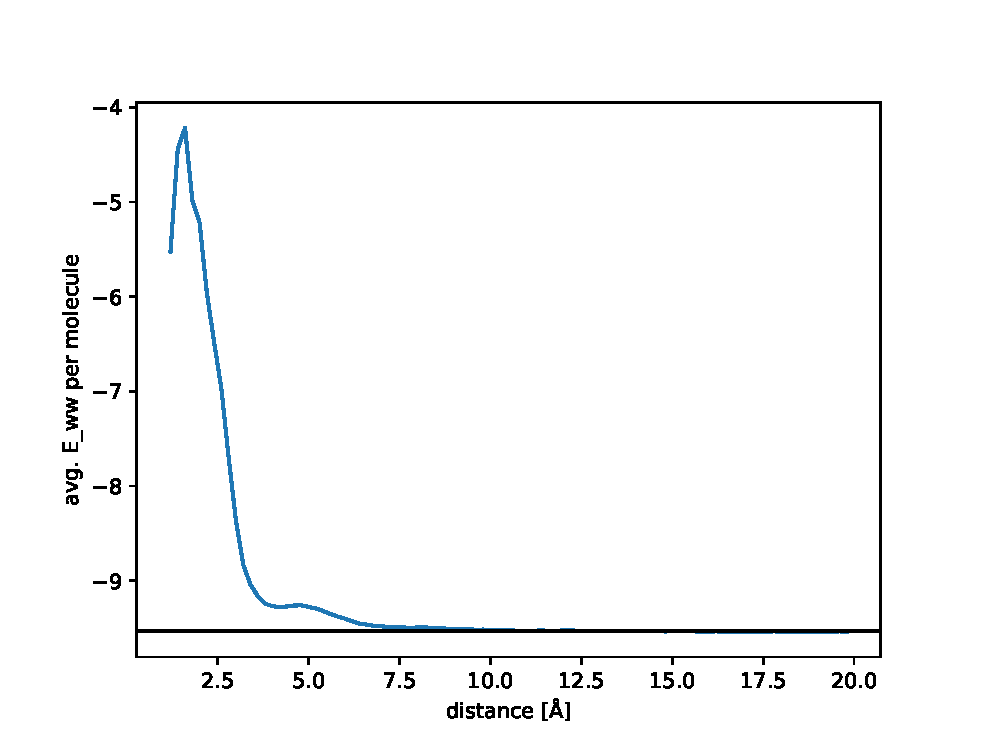
\includegraphics[width=0.8\linewidth]{figures/Eww_convergence.eps}
	\caption{Convergence of $E_{ww}$ in the complex calculation with increasing distance to the solute molecule (streptavidin-biotin). The horizontal line shows the automatically computed reference energy.}\label{fig_ewwref}
\end{figure}
After choosing an appropriate reference value, we need to subtract this value from $E_{ww}$.
Make sure to subtract the reference from the normalized (\_norm) data.
In \software{gisttools}, this is done simply by setting \inlinecode{gist.eww\_ref}.
Now, sum all free energy contributions to obtain the spatially resolved $\dgsolv$.
In \software{gisttools}, this is done automatically and can be accessed using the \inlinecode{A\_dens} and \inlinecode{A\_norm} data rows.

\newcommand{\coordinate}{\mathbf{r}}
\begin{equation}
	\dgsolv(\coordinate) = \Delta E_{ww}(\coordinate) + \Delta E_{sw}(\coordinate) - T\Delta S^\text{six}(\coordinate)
\end{equation}
%In \software{gistpp}, use the \inlinecode{add} command, with the same syntax as the \inlinecode{div} command used above.
After that, check whether your free energy contributions become negligible far away from the solute molecule.
In a plot like Figure~\ref{fig_ewwref} based on the \inlinecode{A\_dens} column, the values should tend to zero.
However, it is more informative to plot the cumulative free energy contribution against the distance to the solute molecule, to check the convergence (see Figure~\ref{fig_radial_convergence}).
If the curve flattens out, the converged value is your final $\dgsolv$\@.
If the curve diverges even for large integration distances you might need to tweak the $E_{ww}$ reference, or introduce a reference value for the entropy.

\begin{lstlisting}[style=python]
from gisttools.gist import load_gist_file
import matplotlib.pyplot as plt
import numpy as np
# adapt eww_ref according to the used solvent model! 
gist = load_gist_file('gist.dat',
    struct='solute-centered.pdb', eww_ref=-9.533)
bins, (dg, esw, eww, s) = gist.rdf(
    ['A_dens', 'Esw_dens', 'Eww_dens', 'dTSsix_dens'],
    bins=100, rmax=20., normalize='none')
plt.plot(bins, np.cumsum(eww), label='Eww')
plt.plot(bins, np.cumsum(esw), label='Esw')
plt.plot(bins, np.cumsum(dg), label='dG')
plt.plot(bins, np.cumsum(s), label='dS')
plt.legend()
plt.xlabel("distance cutoff []")
plt.ylabel("free energy contribution [kcal/mol]")
\end{lstlisting}
The expected output of this code is shown in Figure~\ref{fig_radial_convergence}.
Especially the solvent-solvent energy is not perfectly flat, indicating that the reference value is not optimal.
%but is also complicated because the solute is charged.
Both the entropy and $E_{sw}$ can be considered converged around \SI{10}{\angstrom}.
While this is not true for $E_{ww}$, we will see below that the energy difference upon binding converges more readily than its individual contributions.

\begin{figure}
	\centering
	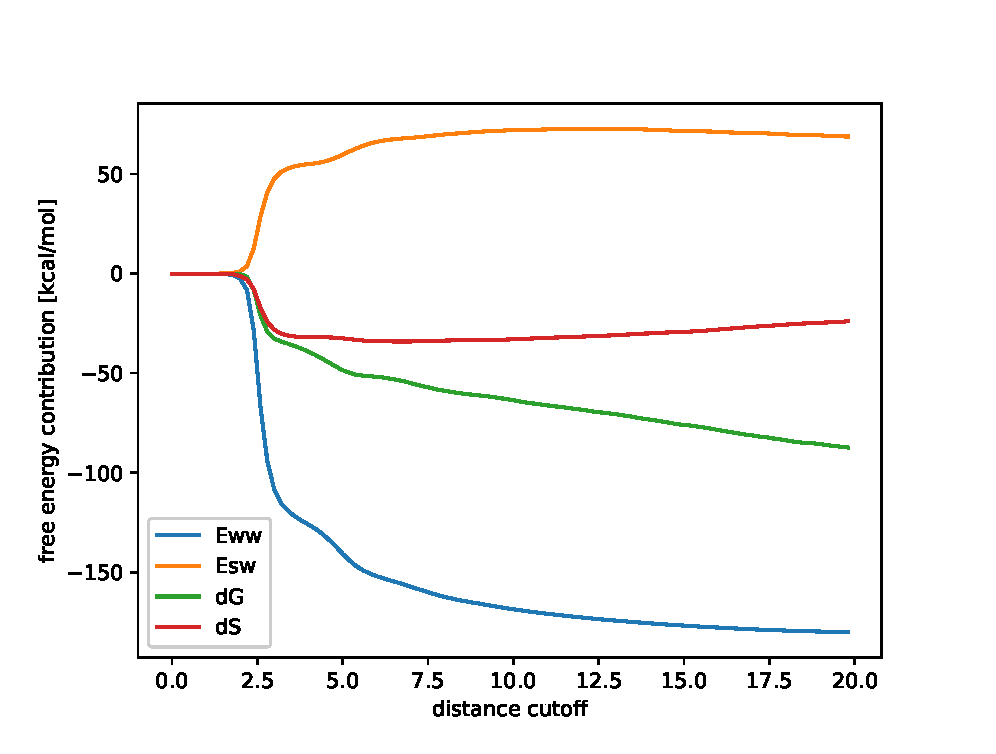
\includegraphics[width=0.8\linewidth]{figures/A_E_S_convergence.eps}
	\caption{Convergence of $\dgsolv$ and its contributions with increasing distance to the solute molecule. All quantities are cumulative, i.e., summed up to the respective radius. Computed from the biotin calculation.}\label{fig_radial_convergence}
\end{figure}

\subsubsection{Visualizing $\dgsolv$}
Next, we visualize the 3-dimensional contributions to the free energy of hydration, as well as the entropy and enthalpy contributions.
You can use PyMol\cite{pymol} or VMD\cite{vmd} to visualize the .dx files from GIST\@.
With \software{gisttools}, you can create one using e.g., \inlinecode{gist.save\_dx('A\_dens', 'A\_dens.dx')}.
It might also be interesting to visualize the average energy of a water solvent molecule at each grid voxel.
This quantity is given by $2E_{ww} + E_{sw}$.
The energy referencing leads to non-zero normalized values where the population is zero.
While this is irrelevant for further post-processing, it is advantageous for visualization to set those empty regions to zero.
An OpenDX file can be produced using \software{gisttools} as follows:

\begin{lstlisting}[style=python]
import gisttools as gt
gist = gt.gist.load_gist_file('gist.dat',
    struct='solute-centered.pdb', eww_ref=-9.533)
gist['E_norm'] = gist['Eww_norm'] * 2 + gist['Esw_norm']
gist.loc[gist['population'] == 0, 'E_norm'] = 0
gist.save_dx('E_norm', 'gist-E-per-mol-norm.dx')
\end{lstlisting}
The OpenDX files can then be imported into your molecular viewer of choice.
A visualization of entropy and energy contributions to the free energy of solvation of the streptavidin binding pocket is shown in Figure~\ref{fig_binding_pocket_pymol}. 
PyMOL input scripts to generate such visualizations are available in the GitHub repository for this tutorial.

\begin{figure}
	\centering
	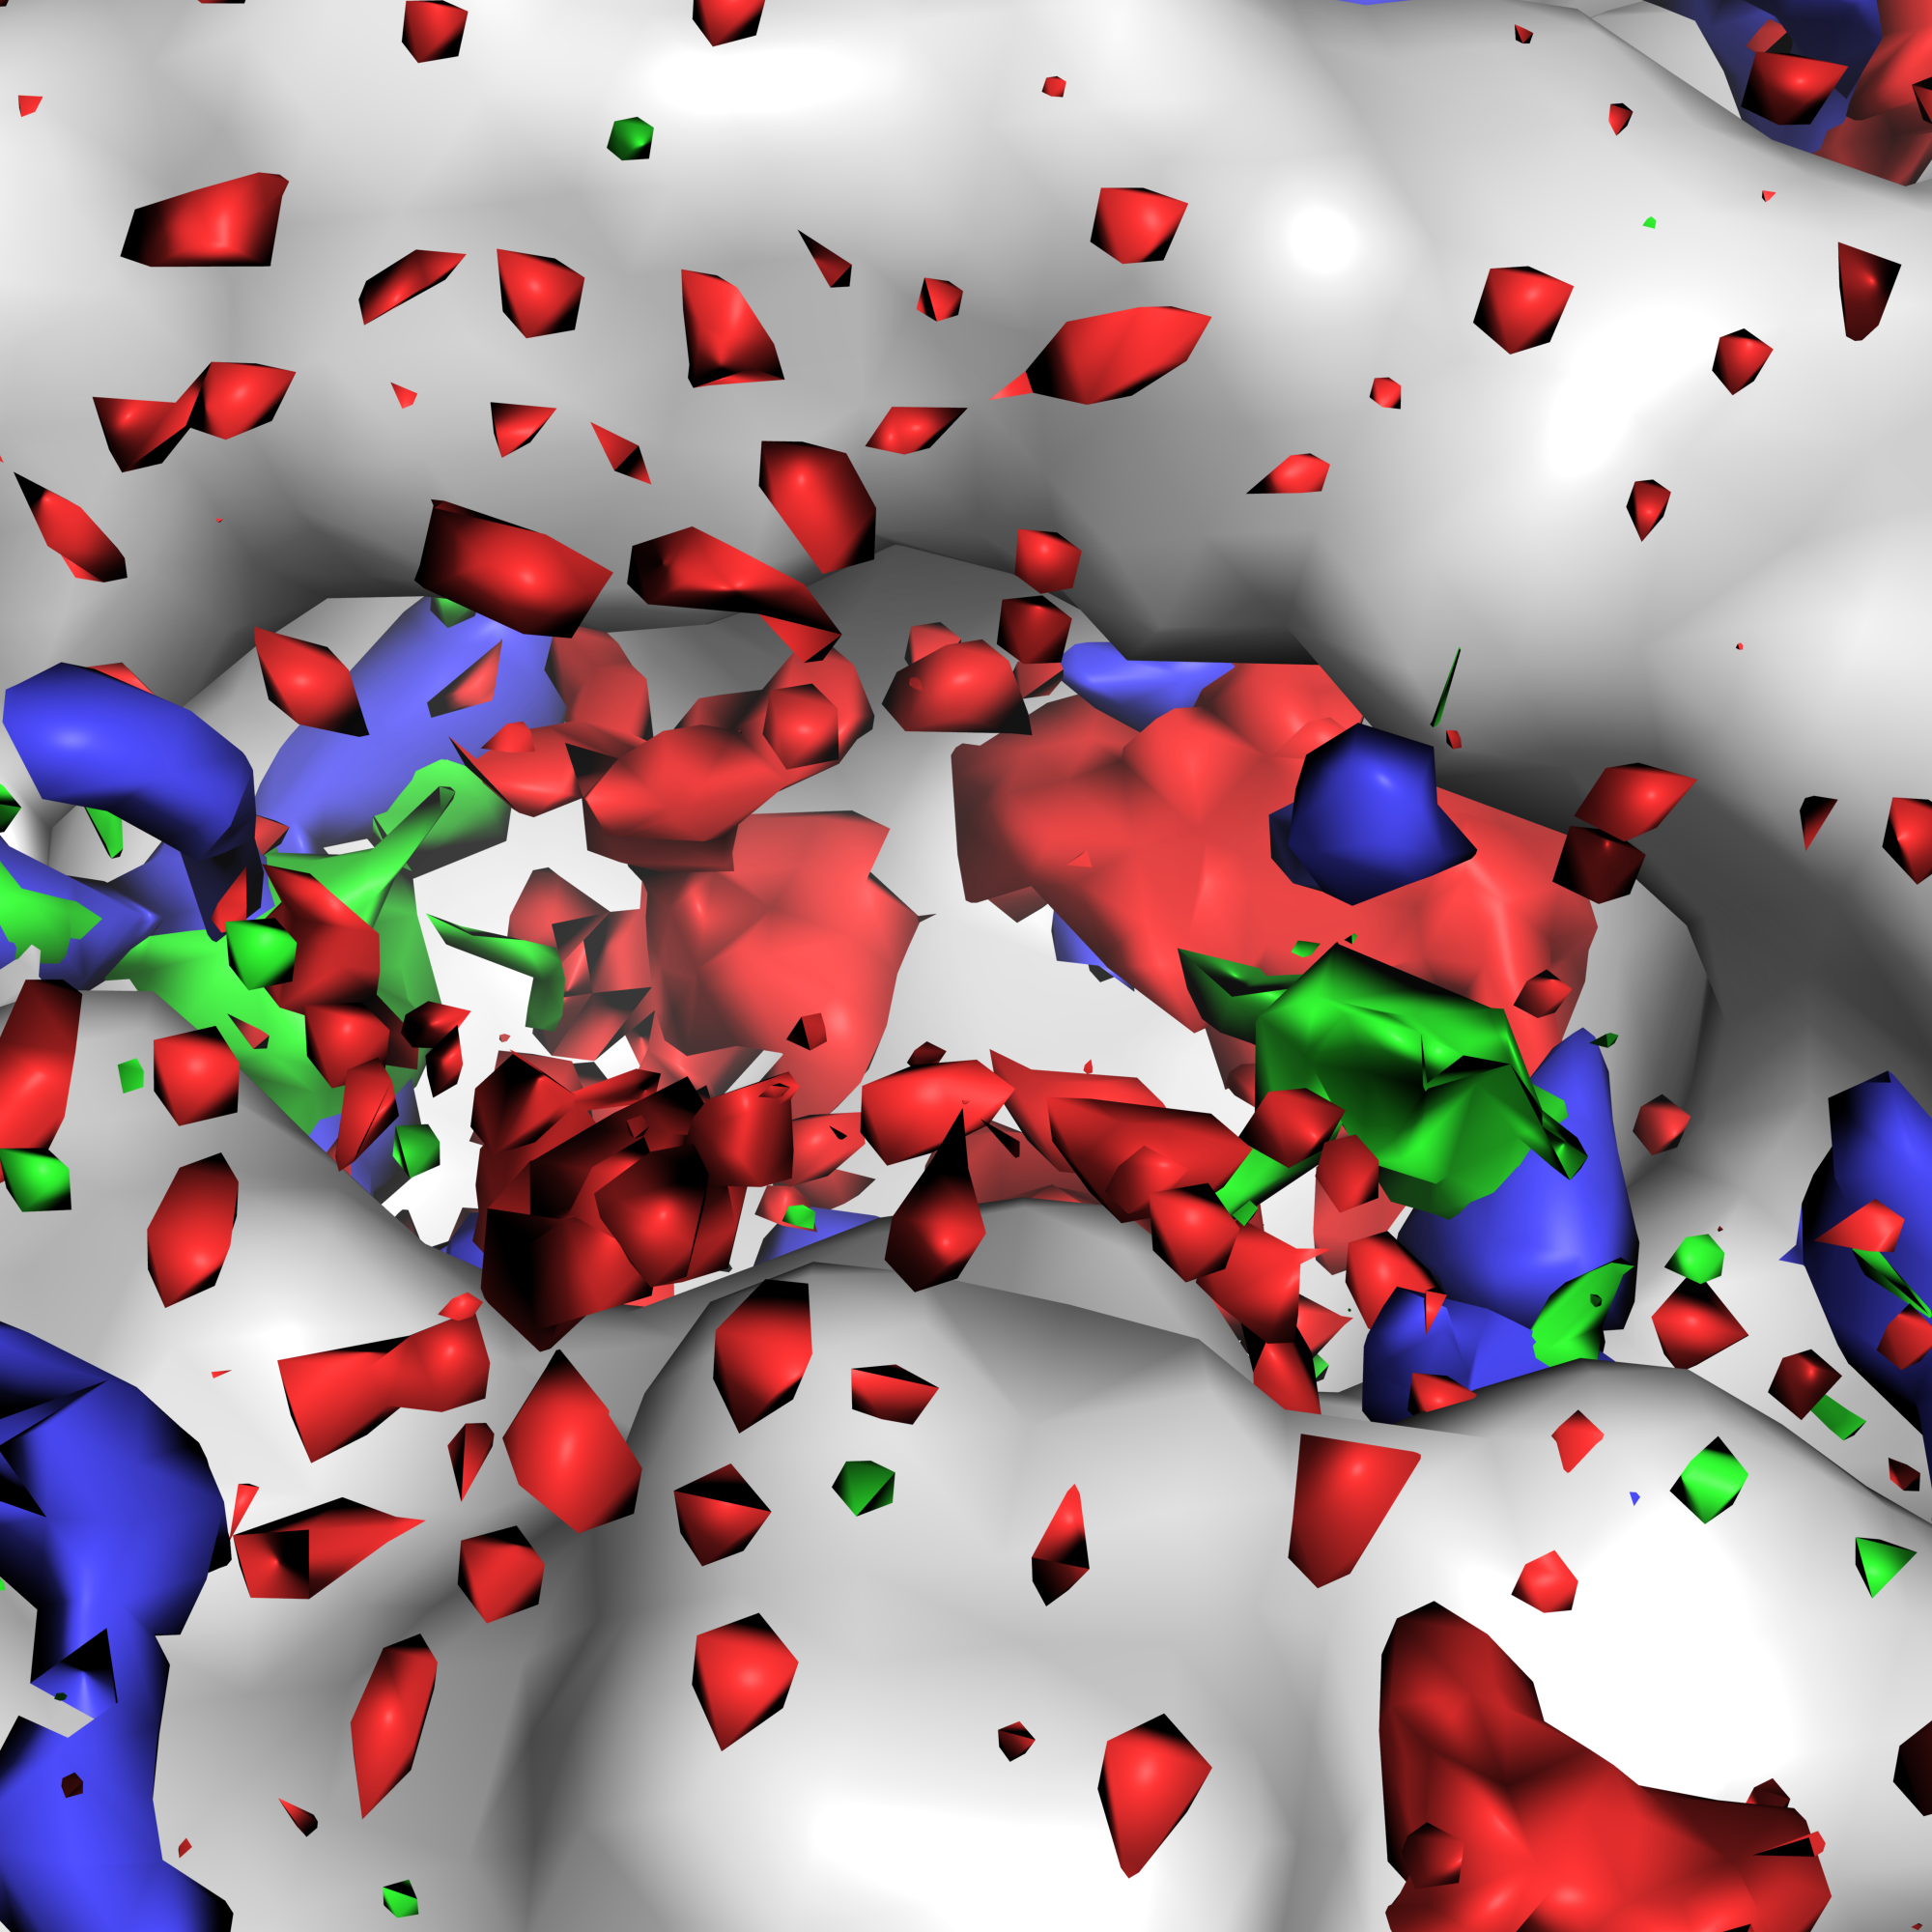
\includegraphics[width=0.8\linewidth]{figures/binding_pocket_norm_quants.png}
	\caption{Free energy contributions in the streptavidin binding pocket. Red: high solvent energy (at +2.5 
	kcal/mol/molecule). Green: low solvent energy (at -2.5 kcal/mol/molecule). Blue: low solvent entropy $T\Delta S^{six}$ 
	(at -2.5 kcal/mol/molecule).}\label{fig_binding_pocket_pymol}
\end{figure}

\subsubsection{Contribution of Hydration to Binding}
\label{sec:binding_contributions}
In the next step, calculate the $\dgsolv$ contributions around biotin in each system (biotin, streptavidin, and complex).
Note that our integration region does not fully reach into bulk, and some of the boundary regions are close to streptavidin. 
Therefore, our results for each system will depend on the exact position of the integration boundary. 
To avoid inconsistencies, it is important to choose exactly the same integration region for each system.
Although we kept the systems rigid, the center of mass might have been shifted during pressure equilibration.
Therefore, we align the complex structure to streptavidin and use the shifted biotin coordinates to define the integration region.
We recommend using a \software{Jupyter Notebook} for the following analyses.
Load the files and double check the frame numbers and reference density.
\begin{lstlisting}[style=python]
import numpy as np
from gisttools.gist import load_gist_file
import matplotlib.pyplot as plt

compl = load_gist_file('complex/gist/gist.dat', \
    struct='complex/gist/solute-centered.pdb')
print(compl.n_frames, compl.rho0)
biotin = load_gist_file('biotin/gist/gist.dat', \
    struct='biotin/gist/solute-centered.pdb')
print(biotin.n_frames, biotin.rho0)
strept = load_gist_file('streptavidin/gist/gist.dat', \
    struct='streptavidin/gist/solute-centered.pdb')
print(strept.n_frames, strept.rho0)
\end{lstlisting}
Assign reference energies and check them for plausibility.

\begin{lstlisting}[style=python]
biotin.eww_ref = biotin.detect_reference_value()
print('Biotin:', biotin.eww_ref)
strept.eww_ref = strept.detect_reference_value()
print('Streptavidin:', strept.eww_ref)
compl.eww_ref = compl.detect_reference_value()
print('Complex:', compl.eww_ref)
\end{lstlisting}
Subtract a reference entropy from the \inlinecode{dTSsix} columns.

\begin{lstlisting}[style=python]
def reference_entropy(gf):
    if 'dTSsix_unref_norm' not in gf.data.columns:
        gf['dTSsix_unref_norm'] = gf['dTSsix_norm']
        gf['dTSsix_unref_dens'] = gf['dTSsix_dens']
    gf['dTSsix_norm'] = gf['dTSsix_unref_norm'] \
        - gf.detect_reference_value('dTSsix_unref_dens')
    gf['dTSsix_dens'] = gf.norm2dens(gf['dTSsix_norm'])
reference_entropy(biotin)
reference_entropy(strept)
reference_entropy(compl)
\end{lstlisting}
Compute the atom positions that define the integration region.
For the streptavidin integral, we align the complex structure onto streptavidin and then use the biotin positions as centers. Note that we use \software{mdtraj} here, since \software{gisttools} stores the reference structure as an \software{mdtraj} \inlinecode{Trajectory} object.
Here, we compute the histogram of the contributions of single properties to assess the convergence.

\begin{lstlisting}[style=python]
import mdtraj as md
col = 'dTSsix_dens'
def select(traj, sel):
    # Slice a Trajectory by selection mask.
    return traj.atom_slice(traj.top.select(sel))
# we multiply by 10 to convert nm to Angstrom.
biotin_mask = 'resname BTN and not element H'
strept_mask = 'not resname BTN and not resname WAT and not element H'
compl_x = select(compl.struct, biotin_mask).xyz[0] * 10.
biotin_x = select(biotin.struct, biotin_mask).xyz[0]*10.
aligned = compl.struct[:].superpose(strept.struct, \
    atom_indices=strept.struct.top.select(strept_mask))
aligned = select(aligned, biotin_mask)
strept_x = aligned.xyz[0] * 10.

bins, biotin_rdf = biotin.rdf( \
    col, centers=biotin_x, bins=100, rmax=24)
bins, strept_rdf = strept.rdf( \
    col, centers=strept_x, bins=100, rmax=24)
bins, compl_rdf = compl.rdf( \
    col, centers=compl_x, bins=100, rmax=24)
\end{lstlisting}
Now, subtract the monomer histograms from the complex, and compute the sum of your property within some cutoff distance to the solute.
If you also visualize the individual histograms, you will notice that the difference converges much better with increasing radius than the single contributions.

\begin{lstlisting}[style=python]
difference = compl_rdf - biotin_rdf - strept_rdf
cutoff = 12
integral = difference[bins < cutoff].sum()
print('Integral = {}'.format(integral))
plt.plot(bins, np.cumsum(difference))
plt.axvline(cutoff)
plt.xlabel('distance to biotin [Å]')
plt.ylabel('dG contribution [kcal/mol]')
\end{lstlisting}
Finally, you can also plot the difference between the complex and monomer contributions against the distance to biotin, using the complex coordinates for the holo structure:

\begin{lstlisting}[style=python]
fig, (ax1, ax2) = plt.subplots(1, 2, figsize=(8, 4))
cutoff = 12
ax1.plot(bins, np.cumsum(biotin_rdf), label='biotin')
ax1.plot(
    bins, np.cumsum(strept_rdf), label='streptavidin')
ax1.plot(bins, np.cumsum(compl_rdf), label='complex')
ax1.legend()
ax1.axvline(cutoff, color='k', linestyle='--')
ax1.set_xlabel('distance to biotin [Å]')
ax1.set_ylabel('$\Delta G$ contributions [Å]')
ax1.grid()

difference = compl_rdf - biotin_rdf - strept_rdf
ax2.plot(bins, np.cumsum(difference))
ax2.axvline(cutoff, color='k', linestyle='--')
ax2.set_xlabel('distance to biotin [Å]')
ax2.set_ylabel('$\Delta \Delta G$ [kcal/mol]')
ax2.grid()
plt.show()
\end{lstlisting}
The expected result is shown in Figure~\ref{fig-dg-sums}.
\begin{figure}[H]
	\centering
	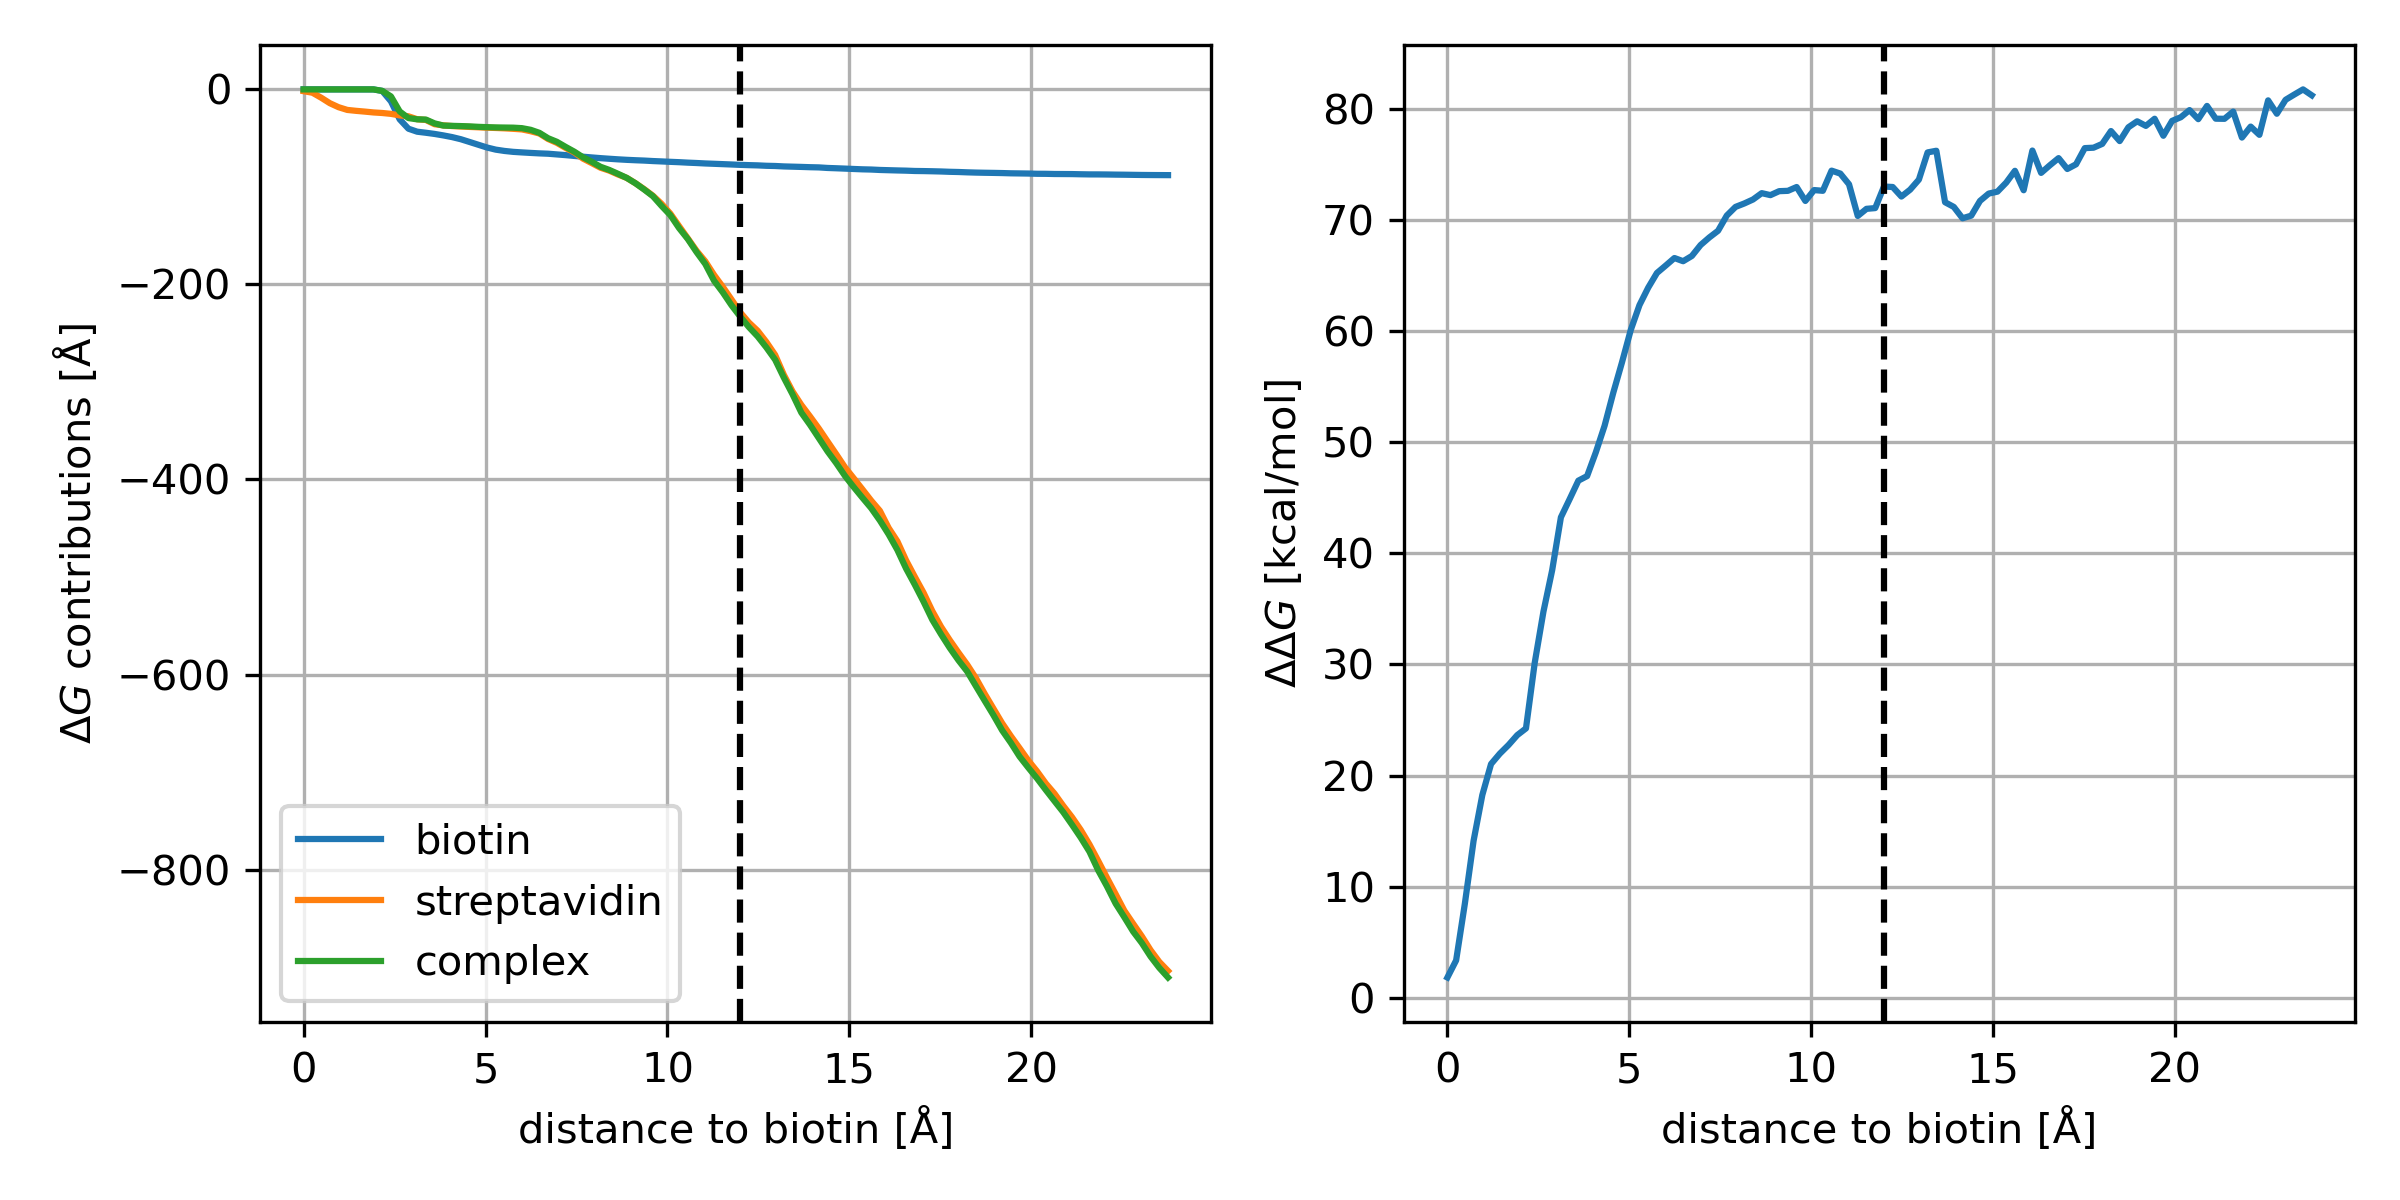
\includegraphics[width=1.0\linewidth]{figures/deltaG-difference.png}
	\caption{Left: $\dgsolv$ contributions around the location of biotin in the binding pocket, evaluated in the biotin, streptavidin, and complex systems. Each line represents a cumulative sum plotted against the distance to biotin. Right: The hydration contribution to binding, evaluated as the difference between the lines in the left panel. The vertical dashed line is at \SI{12}{\angstrom} and represents the chosen integration cutoff.}\label{fig-dg-sums}
\end{figure}
Compute the energy (\inlinecode{Eall}) and entropy (\inlinecode{dTSsix}) contributions separately.
 To make this easier, gisttool includes a function to integrate in a radius around atom centers:
\begin{lstlisting}[style=python]
import pandas as pd
centers = {'biotin': biotin_x, 
    'strept': strept_x, 
    'compl': compl_x}
gist_objs = {'biotin': biotin, 
    'strept': strept, 
    'compl': compl}
cols = ['Eall_dens','dTSsix_dens']
rmax = 12
results = {
    name: gist.integrate_around(
    cols, rmax, centers[name])
    for name, gist in gist_objs.items()}
print(pd.DataFrame(results))
\end{lstlisting}
You will find that the energy disfavors binding, because we do not yet include the interaction energy between biotin and streptavidin.
Using the \inlinecode{energy} command in \software{cpptraj}, you can compute this interaction energy.
We recommend using PME in combination with PME-GIST, but not with GPU-GIST to be in line with the different ways the energy is calculated in the two GIST methods.
An example \software{cpptraj} is then:
\begin{lstlisting}[style=cpptraj]
parm solvated.parm7
trajin md-01.nc 1 last 100
energy complex ^1,2 # etype pme
energy strept ^1 # etype pme
energy biotin ^2 # etype pme
go
diff = complex[total] - strept[total] - biotin[total]
writedata energy.dat diff complex[total] \
strept[total] biotin[total]
avg(complex[total])
avg(strept[total])
avg(biotin[total])
avg(diff)
\end{lstlisting}
It has been shown \cite{Chen2021,Waibl2022-gist-solvents} that the solvation entropy in water is best approximated by 0.6 times the first order entropy provided by GIST.
So we also compute the scaled entropy and check the effect on the binding affinity.
The expected results are summarized in Table~\ref{tab_dg_monomers_dimer}.


\begin{table}[h]
	\caption{Free energy contributions for the monomers and the dimer in kcal$\cdot$mol$^{-1}$. ``Diff'' is calculated as 
	$E^\text{internal} + \Delta E^\text{GIST} - \Delta S^\text{scaled}$. ``total'' is calculated as 
	``complex''-``streptavidin'' - ``biotin''.}\label{tab_dg_monomers_dimer}
	\small
	\begin{tabular}{@{}lrrrrr@{}}
		\toprule
		System       & $E^{internal}$ & $\Delta E^\textit{GIST}$ & $T\Delta S^\textit{GIST}$ & $T\Delta S^\textit{scaled}$ & Diff \\
		\midrule
		complex      & -1303.4 & -361.2 & -233.1 & -139.9 & -1524.7 \\
		streptavidin & -1180.7 & -360.8 & -242.4 & -145.4 & -1396.1 \\
		biotin       & -24.0   &  -98.1 &  -35.1 &  -21.1 &  -101.0 \\
		\midrule
		total         & -98.7   &   97.7 &   44.4 &   26.6 &   -27.6 \\
		\bottomrule
	\end{tabular}
\end{table}
Even though streptavidin-biotin is known to be a very stable complex, the free solvation energy ($\Delta E^{GIST}-T\Delta S^{scaled}$) favors the dissociation.
This is expected: the binding of biotin to streptavidin is facilitated over a large number of H-bonds and over polar interactions. 
As such, water favourably solvates both biotin and streptavidin and an energetic penalty is paid when displacing the water during the binding process. 
In this case, we find that the changes in the energy of solvation and of the internal energy $\Delta E^{internal}$ more or less cancel out, indicating that binding is largely entropy-driven in this case.
At first, this is surprising, since isothermal titration calorimetry (ITC) of biotin-streptavidin shows strong enthalpic binding contributions \cite{mpye2020-biotin-itc,hyre2006-biotin-itc}.
However, we do not take the conformational transition of the streptavidin binding pocket into account.

Prior computational studies suggest a $\Delta G$ of \SI{-26.6}{\kilo\calorie\per\mole} for the binding of biotin into the closed conformation of streptavidin \cite{Bansal2018-biotin}.
This indicates that our result is in good agreement with literature.
To improve the agreement with ITC measurements, the conformational changes of the binding pocket should be included.

\subsubsection{Further steps}
In this tutorial, we obtained a value for the binding of biotin into the closed conformation of the streptavidin binding pocket.
To investigate the effect of different conformations on the binding affinity, you can perform molecular dynamics simulations of the complex and/or monomers and perform GIST on multiple cluster representatives.
To include the effect of lid closing in the binding process, free energy calculation methods such as umbrella sampling can be used.
To speed up the calculation, smaller GIST grids could be used by focusing on the binding pocket, or by rotating the solute molecule by its principal axes to fit the cuboid grid more exactly.
However, this should be done \emph{before} the MD simulation, since rotating the trajectory damages the periodic box information.
%TODO: Ask Dan if this is still the case

\section{Recent developments}
In recent years, several updates to the original GIST implementation have been published.
The basic functionality of the program, however, has not been changed.
In this chapter, we will shortly present each of those updates.
\subsection{GPU implementation}
In Reference~\cite{Kraml2020}, a GPU implementation of the energy calculation was presented, which typically increases the speed by 1--2 orders of magnitude.
If \software{cpptraj} is compiled with GPU support, the energy calculation uses the GPU automatically, without any additional input.
However, PME-GIST is not supported on the GPU, and no GPU code will be used when specifying \inlinecode{pme}.

\subsection{PME implementation}
In Reference~\cite{Chen2021}, a PME implementation of the GIST energy was presented.
For typical systems, this implementation is slightly slower than GPU-GIST, but much faster than the original CPU code.
Furthermore, PME-GIST offers the best agreement between GIST energies and those observed in an classical MD simulation.
To run PME-GIST, the \inlinecode{pme} flag to \inlinecode{gist} can be used in \software{cpptraj}.
The output will contain two additional columns: \inlinecode{PME\_dens} and \inlinecode{PME\_norm}.
They contain the potential of solute molecule and solvent evaluated at the solvent positions and divided by two.
Furthermore, the \inlinecode{Eww} and \inlinecode{Esw} columns are also computed using PME, and are reported as usual.
For typical use cases, we recommend using \inlinecode{Eww} and \inlinecode{Esw} over the \inlinecode{PME} column.

\subsection{MPI parallelization}
The most recent addition to GIST is the MPI parallelization of both energy and entropy calculations \cite{Roe2023-mpi-gist}.
Since the MPI parallelization is orthogonal to the other improvements, it can be used with both PME or GPU accelerated GIST.
\subsection{GIST with non-water solvents}
In references~\cite{Kraml2020,Kamenik2020-gist-macrocycles,Waibl2022-gist-solvents}, an extension of GIST towards solvents other than water is described.
To run a GIST calculation in a solvent other than water, use \inlinecode{solute} with a \software{cpptraj} selection mask to select the solute molecule.
All other molecules will be treated as solvent.
If there are multiple solvent species, also use the \inlinecode{solventmols} flag as described in Section~\ref{sec-salt-water}. \\
The code will automatically choose three atoms per solvent species to define the solvent orientation, and print this selection to the output.
Sometimes, however, the automatic selection is not optimal.
For instance, in methanol one can either incorporate the C--H bonds or the O--H bond in the selection.
The latter is probably more relevant since it can incorporate hydrogen bonding effects.
Assuming that the alcohol hydrogen atom is called H1, this could be specified as follows:

\begin{lstlisting}[style=cpptraj]
gist gridcntr <x> <y> <z> \
griddim <Nx> <Ny> <Nz> gridspacn <val> \
solute ^1 rigidatoms O1 H1 C1
\end{lstlisting}
Note that the central atom of the \inlinecode{rigidatoms} selection goes first.

\subsection{GIST with salt-water mixtures}
\label{sec-salt-water}
In \cite{Waibl2021-gist-salt}, an extension of GIST was presented that can use salt-water mixtures as a solvent.
This allows treating salting-out effects, although it was shown that the salting-out coefficient is over-predicted by GIST because of the first-order entropy approximation.
Generally, GIST should be able to treat arbitrary solvent mixtures as long as each solvent molecule is sufficiently rigid. \\
In the \software{cpptraj} implementation of GIST, the \inlinecode{solute} keyword specifies which components of the system are treated as a solute molecule.
Everything else will be treated as solvent.
If the solvent contains more than one molecular species, a list of solvent molecule names (i.e., ``\inlinecode{solventmols WAT,NA,CL}'') must be specified.
For each solvent molecule in this list, densities (e.g., \inlinecode{g\_mol\_NA}) and energies (e.g., \inlinecode{Eww\_mol\_NA}) will be computed and written to .dx files.
Note that, e.g., \inlinecode{Esw\_mol\_NA} contains the interactions of every ``\inlinecode{NA}'' solvent molecule with the solute molecule, and \inlinecode{Esw\_mol\_NA} contains the interactions among ``\inlinecode{NA}'' solvent molecules as well as their interactions with all other solvents, divided by 2 to account for double counting.
The entropy will be computed using only the density of the first solvent molecule. \\
For instance, a GIST calculation in salt water, including the first-order water entropy, can be run as follows:

\begin{lstlisting}[style=cpptraj]
gist gridcntr <x> <y> <z> \
griddim <Nx> <Ny> <Nz> gridspacn <val> \
solute !(:WAT,NA,CL) solventmols WAT,NA,CL
\end{lstlisting}
The current implementation of the entropy calculation in \software{cpptraj} requires at least 3 atoms in the main solvent.
Note that the calculation of the reference value is complicated by the introduction of additional solvents.
For an overview of how to correctly handle such calculations, refer to reference \cite{Waibl2021-gist-salt}.
Additionally, to compute the first-order entropy of the ions, as well as an approximate second order entropy, Python code is available on \url{https://github.com/liedllab/second-disorder}.
%TODO: Add recommendations how to handle charges/counterions to text (not necessarily here)
\section{Visualization}
\label{sec:visualization}
\subsection{Visualizing DX files}
A minimal PyMOL input to visualize a dx file is shown here.
This loads an input structure from a file named \inlinecode{streptavidin.pdb} and visualizes the oxygen density at an isolevel of 2 (i.e., twice the reference density).
The expected output is shown in Figure~\ref{fig-streptavidin_gO}.

\begin{lstlisting}[style=pymol]
load output/streptavidin/gist.pdb, streptavidin
as surface
color gray70, streptavidin
load output/streptavidin/gist-gO.dx, gO
isomesh gO_high, gO, 2
color slate, gO_high
\end{lstlisting}
A more sophisticated visualization, including the energy, entropy, and free energy of removing a single water solvent 
molecule, is found in Figure~\ref{fig-binding-pocket}.
\begin{figure}
	\centering
	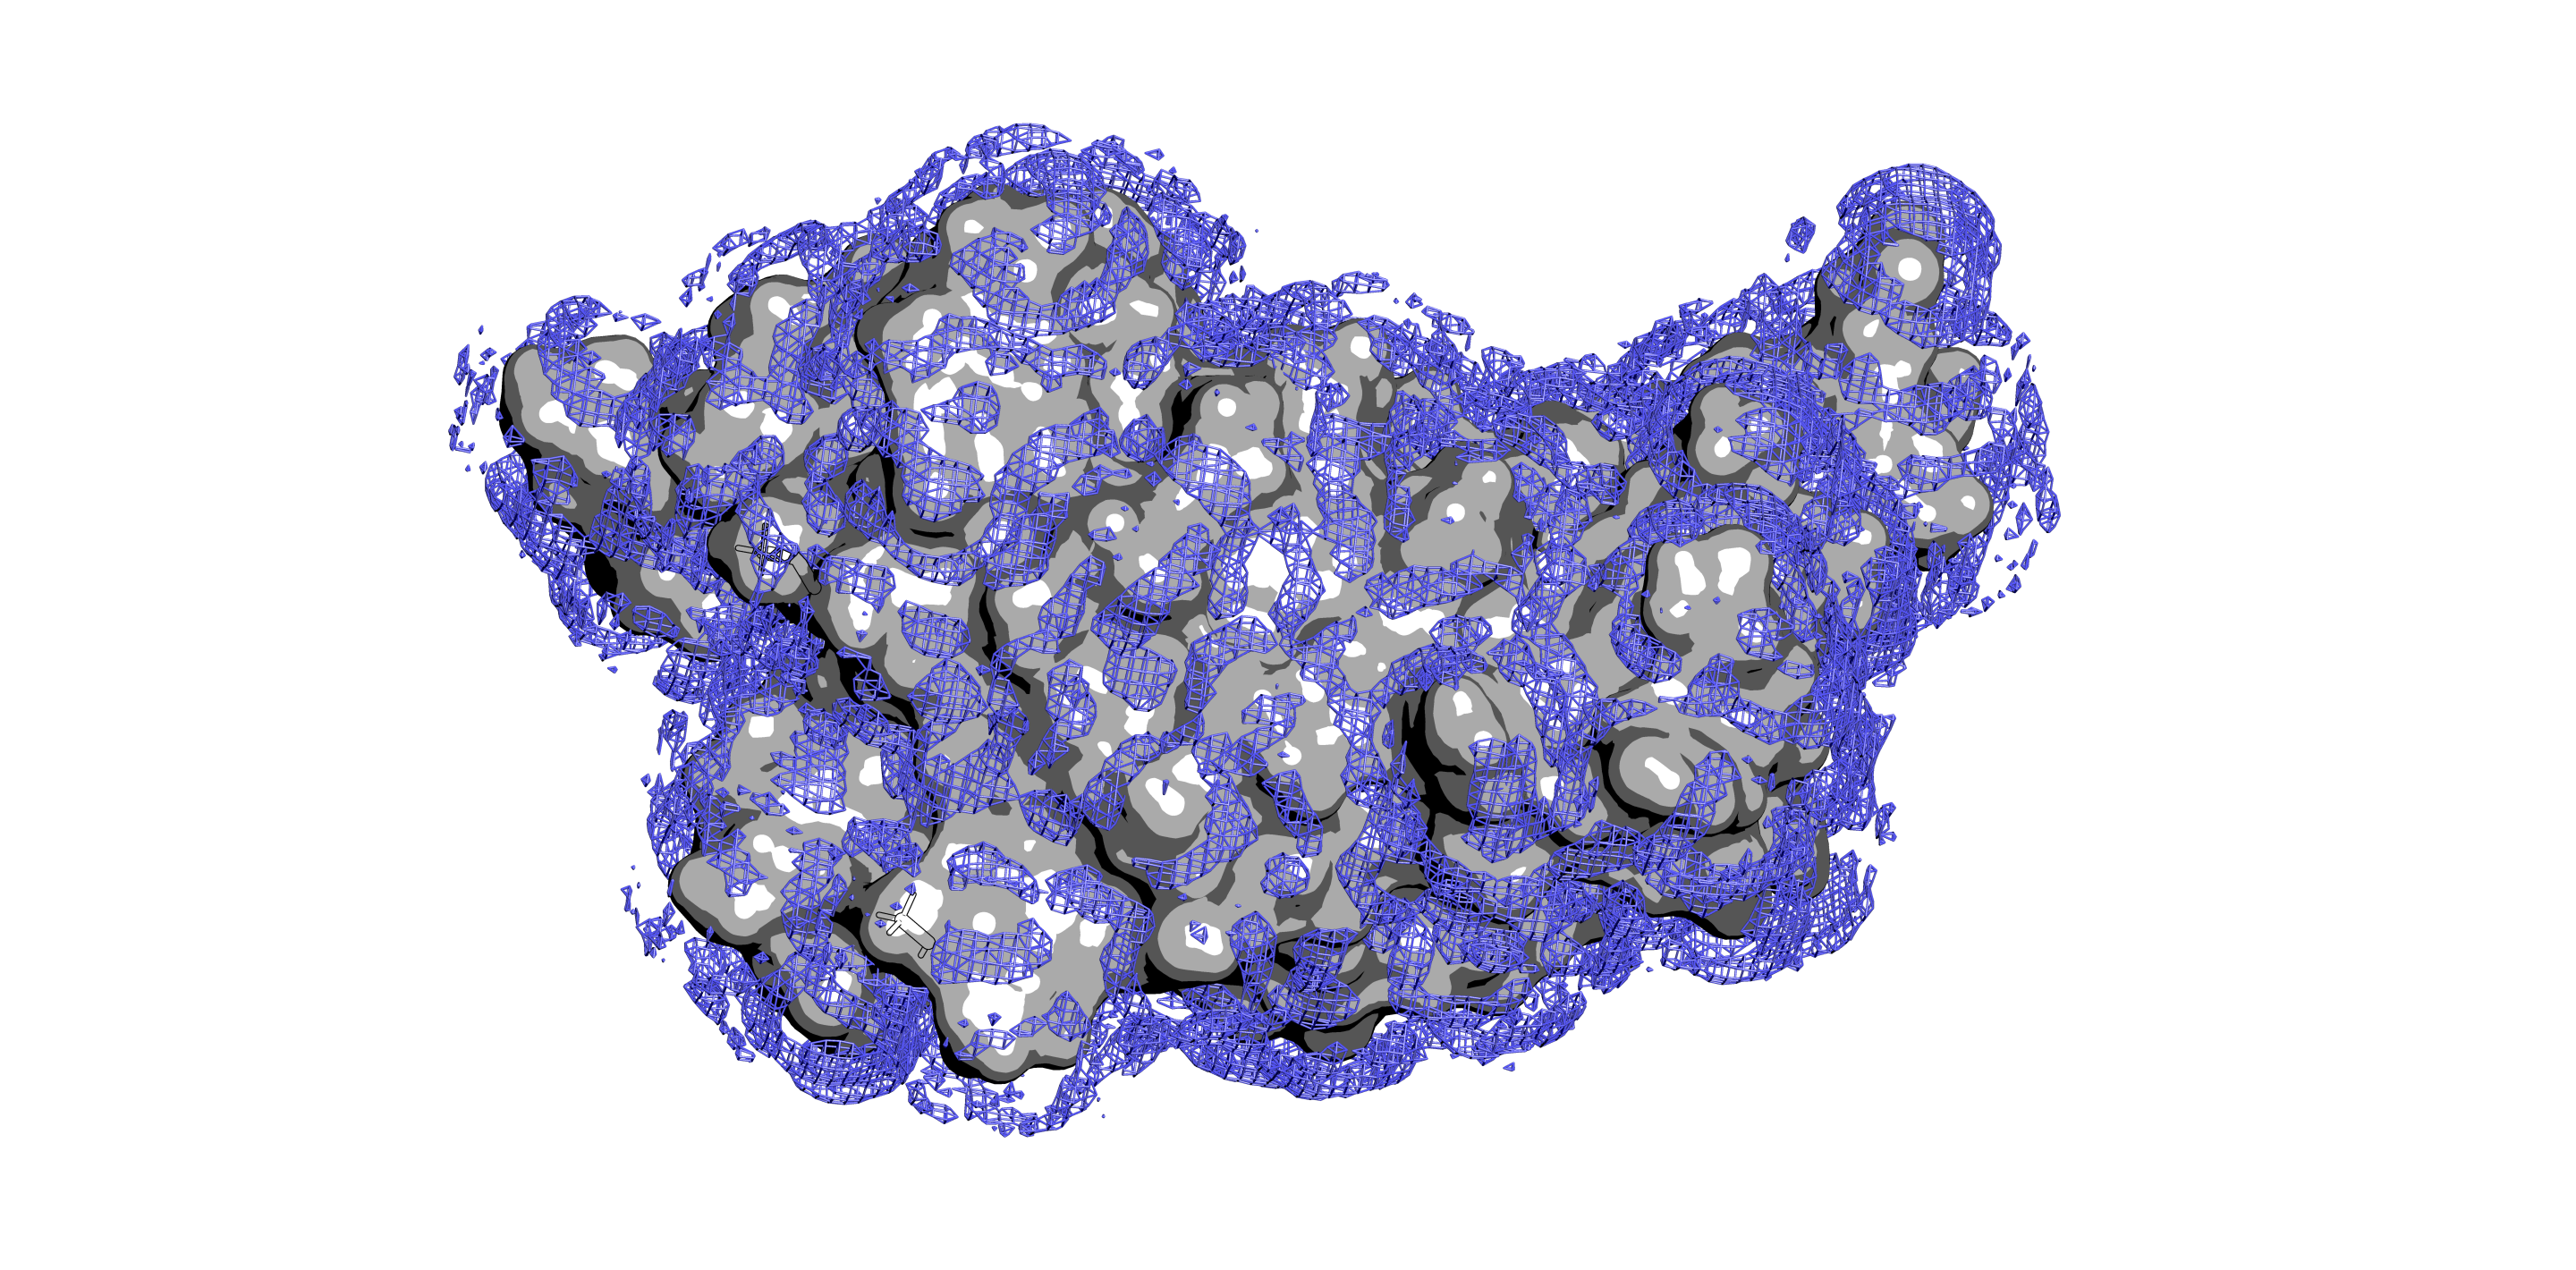
\includegraphics[width=1\linewidth]{figures/streptavidin_gO_high_surf.png}
	\caption{Oxygen density around streptavidin at an isolevel of twice the reference density (i.e., bulk)}
	\label{fig-streptavidin_gO}
\end{figure}
\begin{figure}
	\centering
	\begin{subfigure}[b]{0.45\textwidth}
	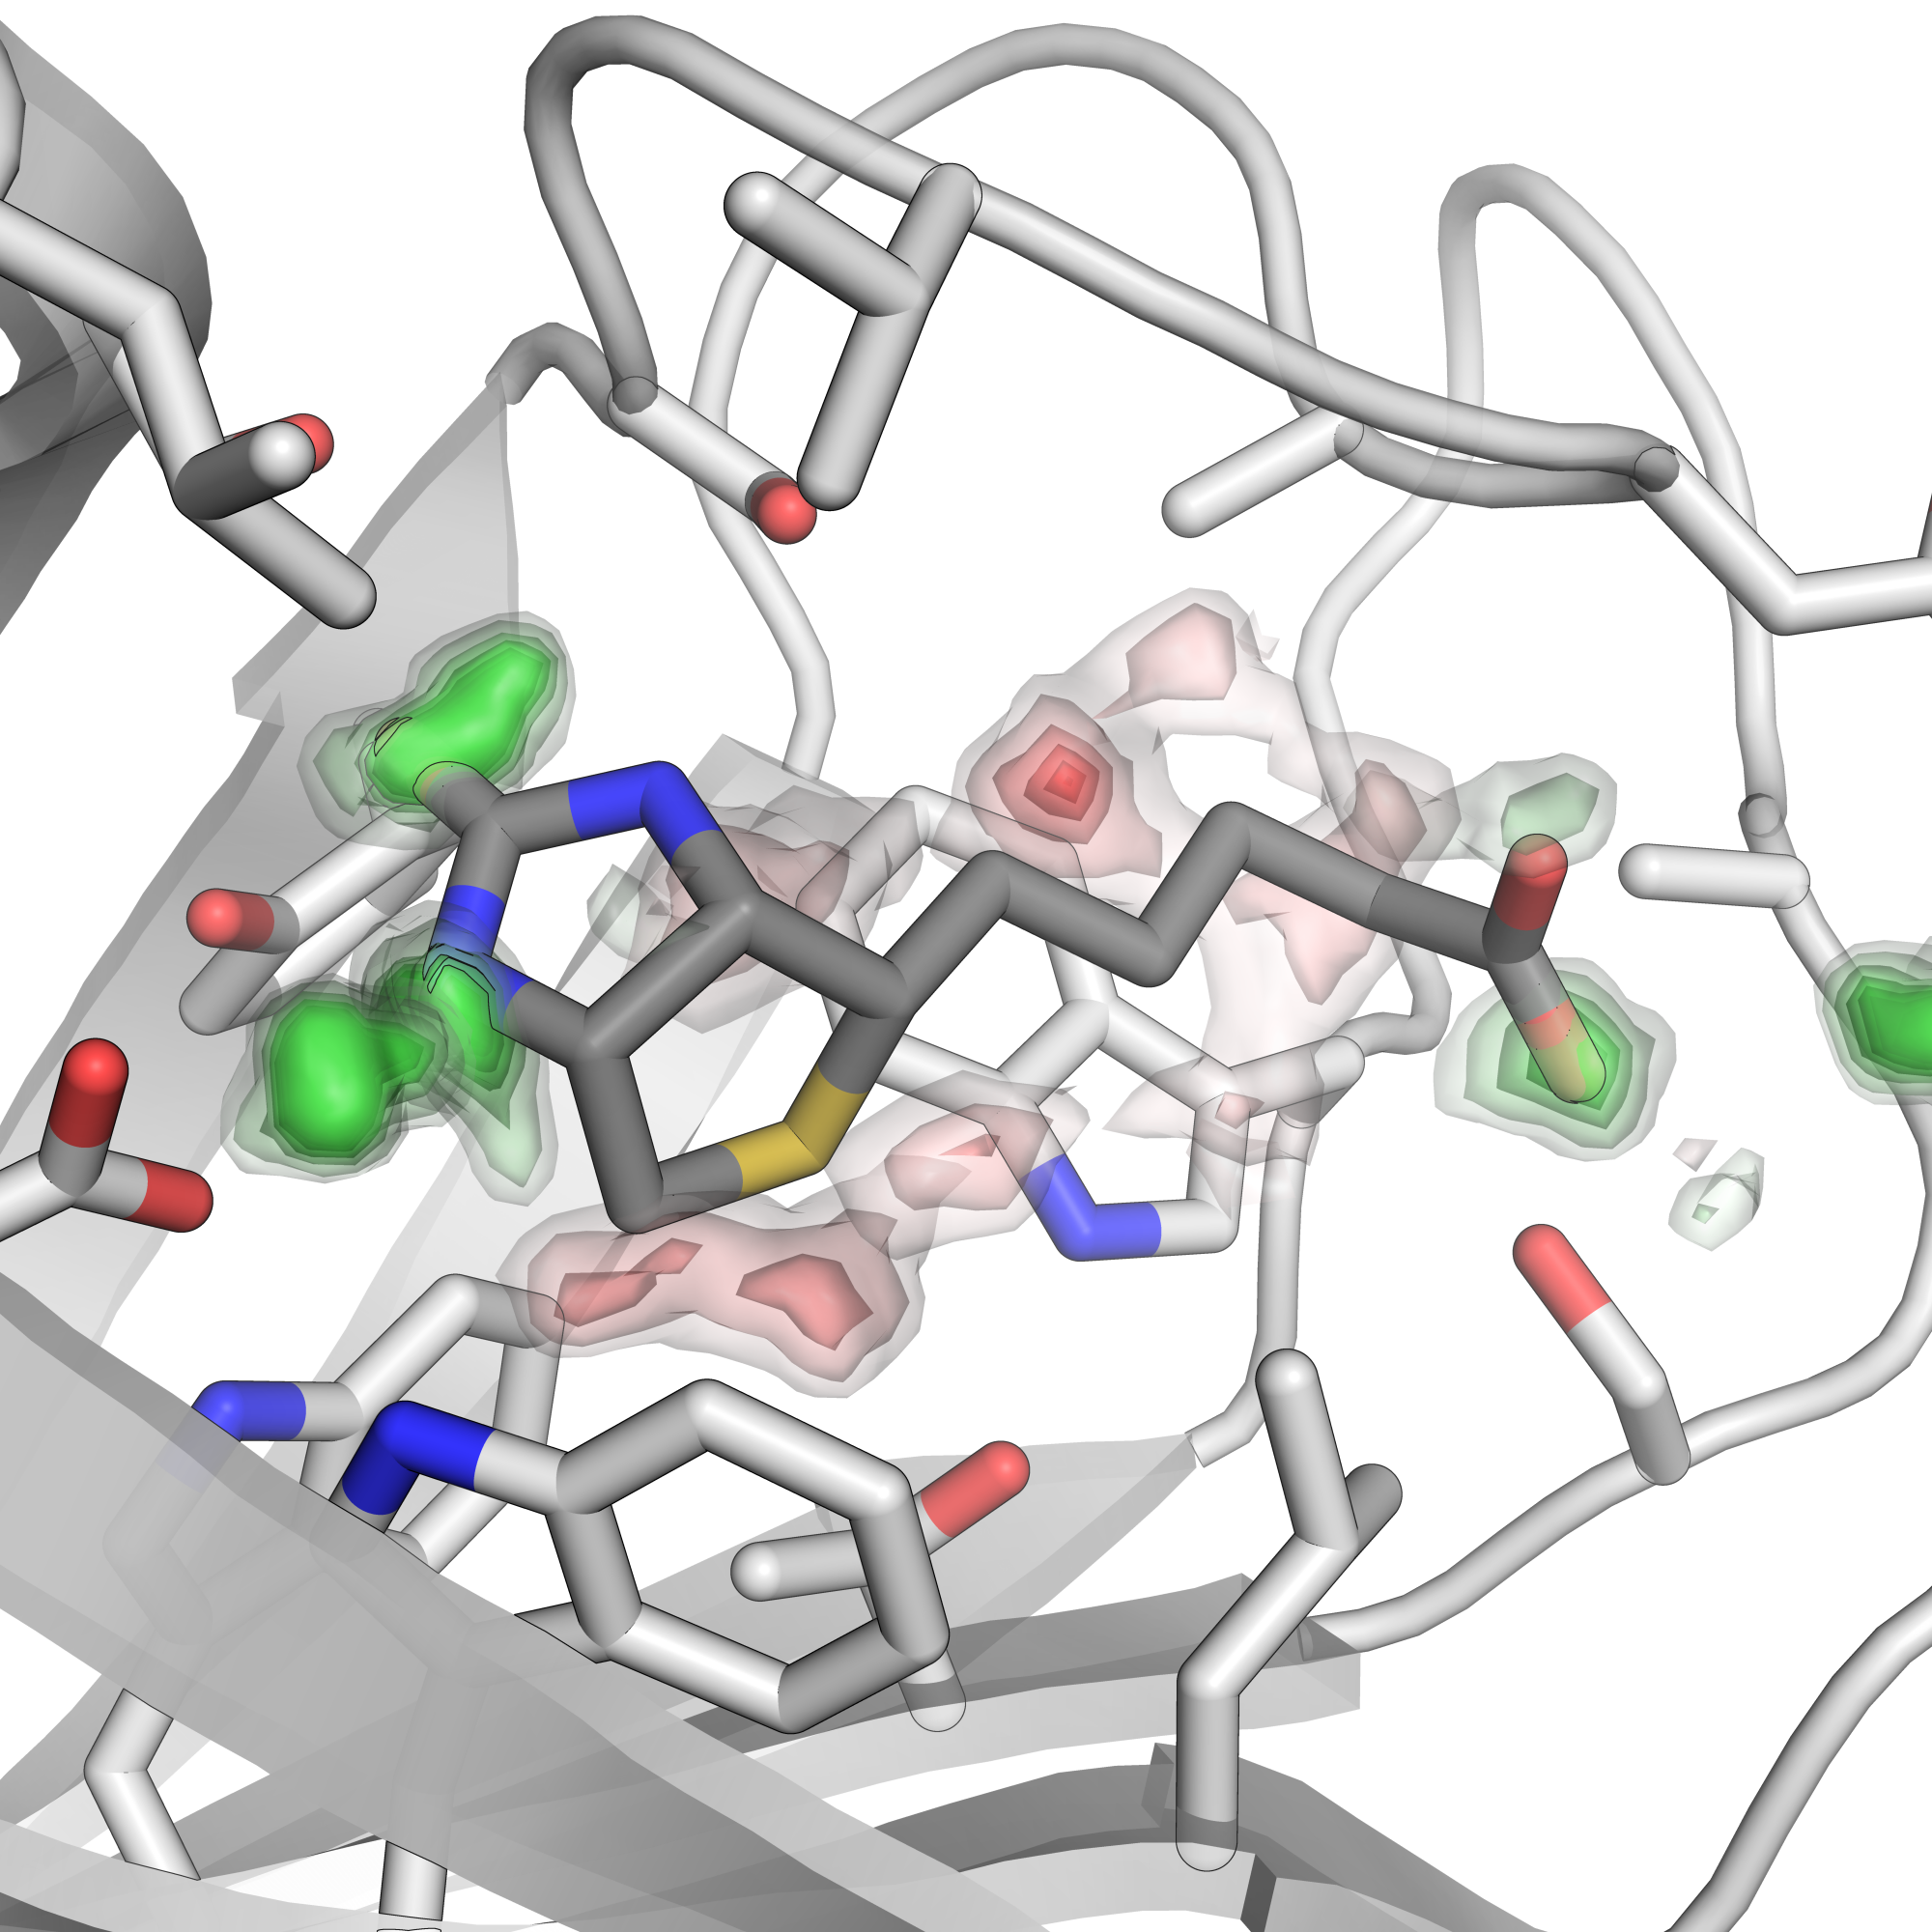
\includegraphics[width=\linewidth]{figures/binding_pocket_E.png}
	\caption{GIST solvent energy (based on $E_{sw} + 2E_{ww}$).}
	\label{fig-binding-pocket-energy}
    \end{subfigure}
	\hfill
	\begin{subfigure}[b]{0.45\textwidth}
		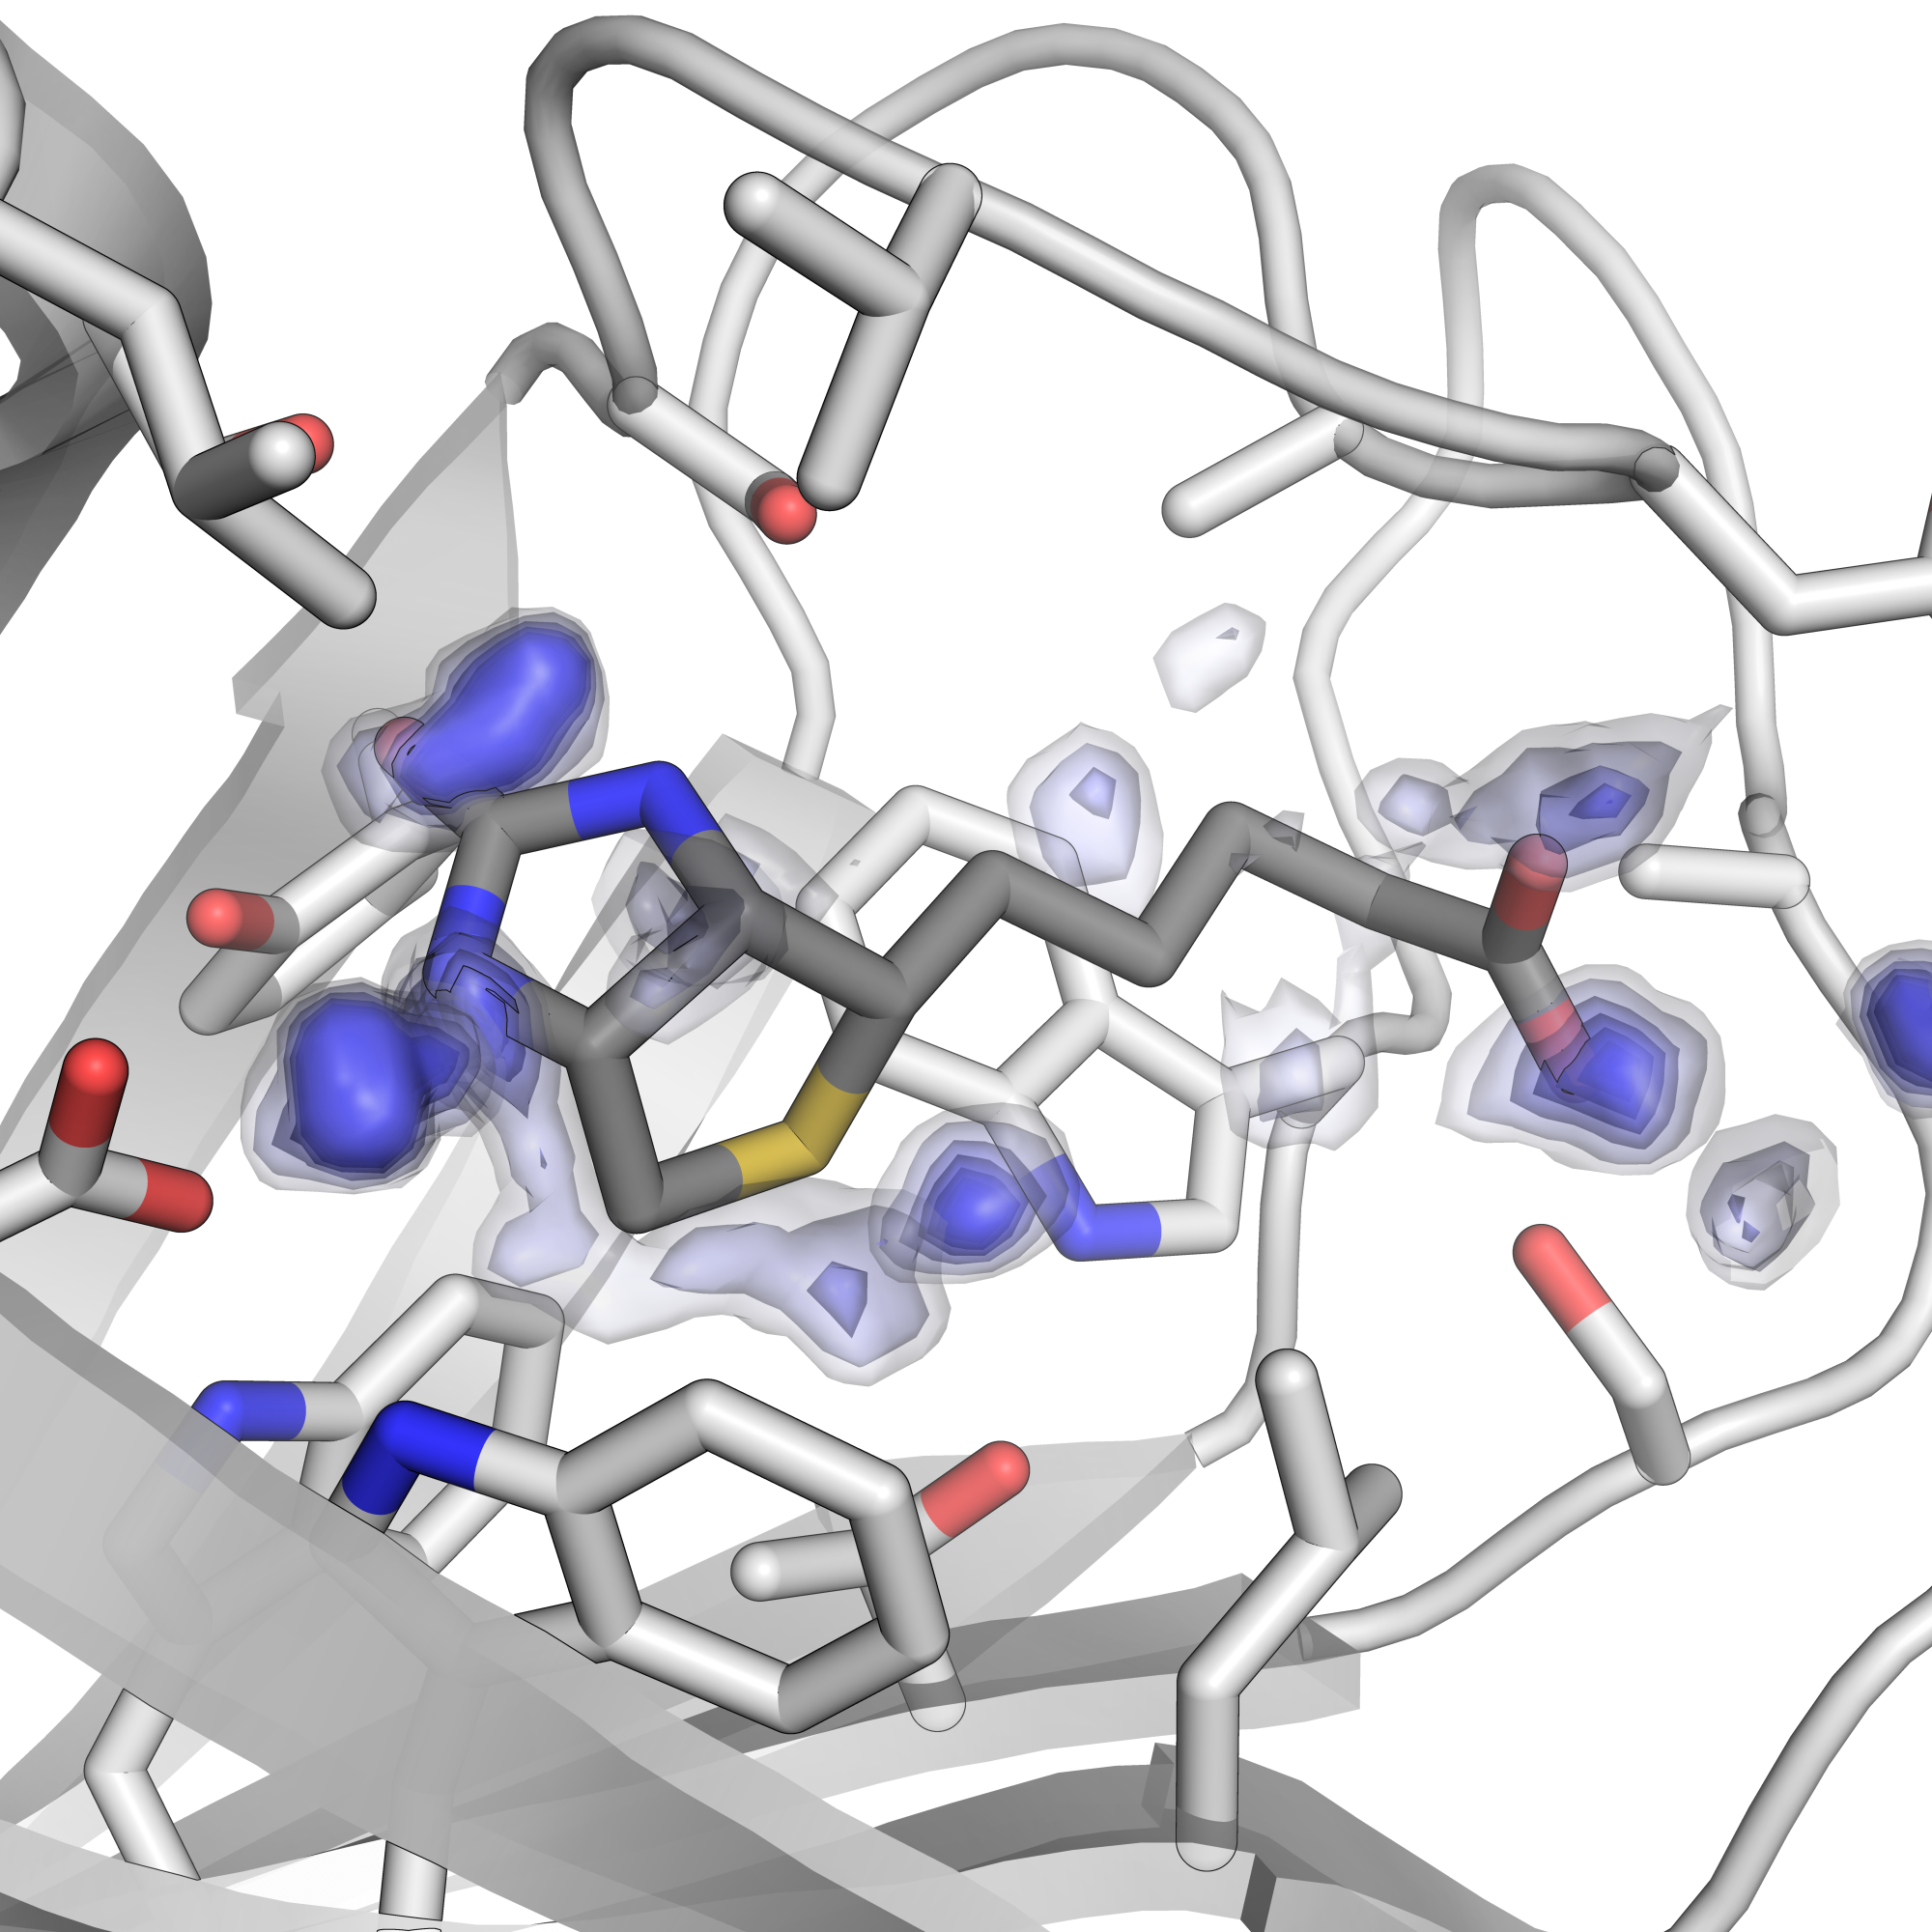
\includegraphics[width=\linewidth]{figures/binding_pocket_S.png}
		\caption{GIST solvent entropy}
		\label{fig-binding-pocket-entropy}
	\end{subfigure}
	\caption{Biotin in the streptavidin binding pocket, with isosurfaces based on the GIST calculation on the holo structure. 
	Isolevels shown are ($\pm$) 0.25, 0.5, 1.0, 1.5, 2.0, 2.5, and 3.0 \si{\kilo\calorie\per\mole\per\cubic\angstrom}, except for 
	the positive energy, where they are divided by two to visually account for its overall lower density. The negative solvent energgy is shown in green, positive solvent energy in red and negative entropy in blue. Only voxels within \SI{4}{\angstrom} of biotin are shown.}
	\label{fig-binding-pocket}
\end{figure}

\subsection{Solvent Accessible Surface (SAS)}
The solvent accessible surface (SAS) represents the interface between regions that are occupied by the solute molecule, and those which can be accessed by the solvent.
GIST provides a very natural way of creating a SAS using an isosurface of the oxygen density \code{gO}.
At a very low isovalue, an isosurface of the water's oxygen or hydrogen shows areas the water can reach, essentially creating a SAS. 
Here, the SAS was generated from a simulation of water around streptavidin without biotin, leaving the binding site solvent-accessible.
The expected output is shown in Figure~\ref{fig-streptavidin_sasa}.

\begin{lstlisting}[style=pymol]
load ../gist.pdb
load ../gist-gO.dx
isomesh sas, gist-gO, 0.1
\end{lstlisting}

\begin{figure}
	\centering
	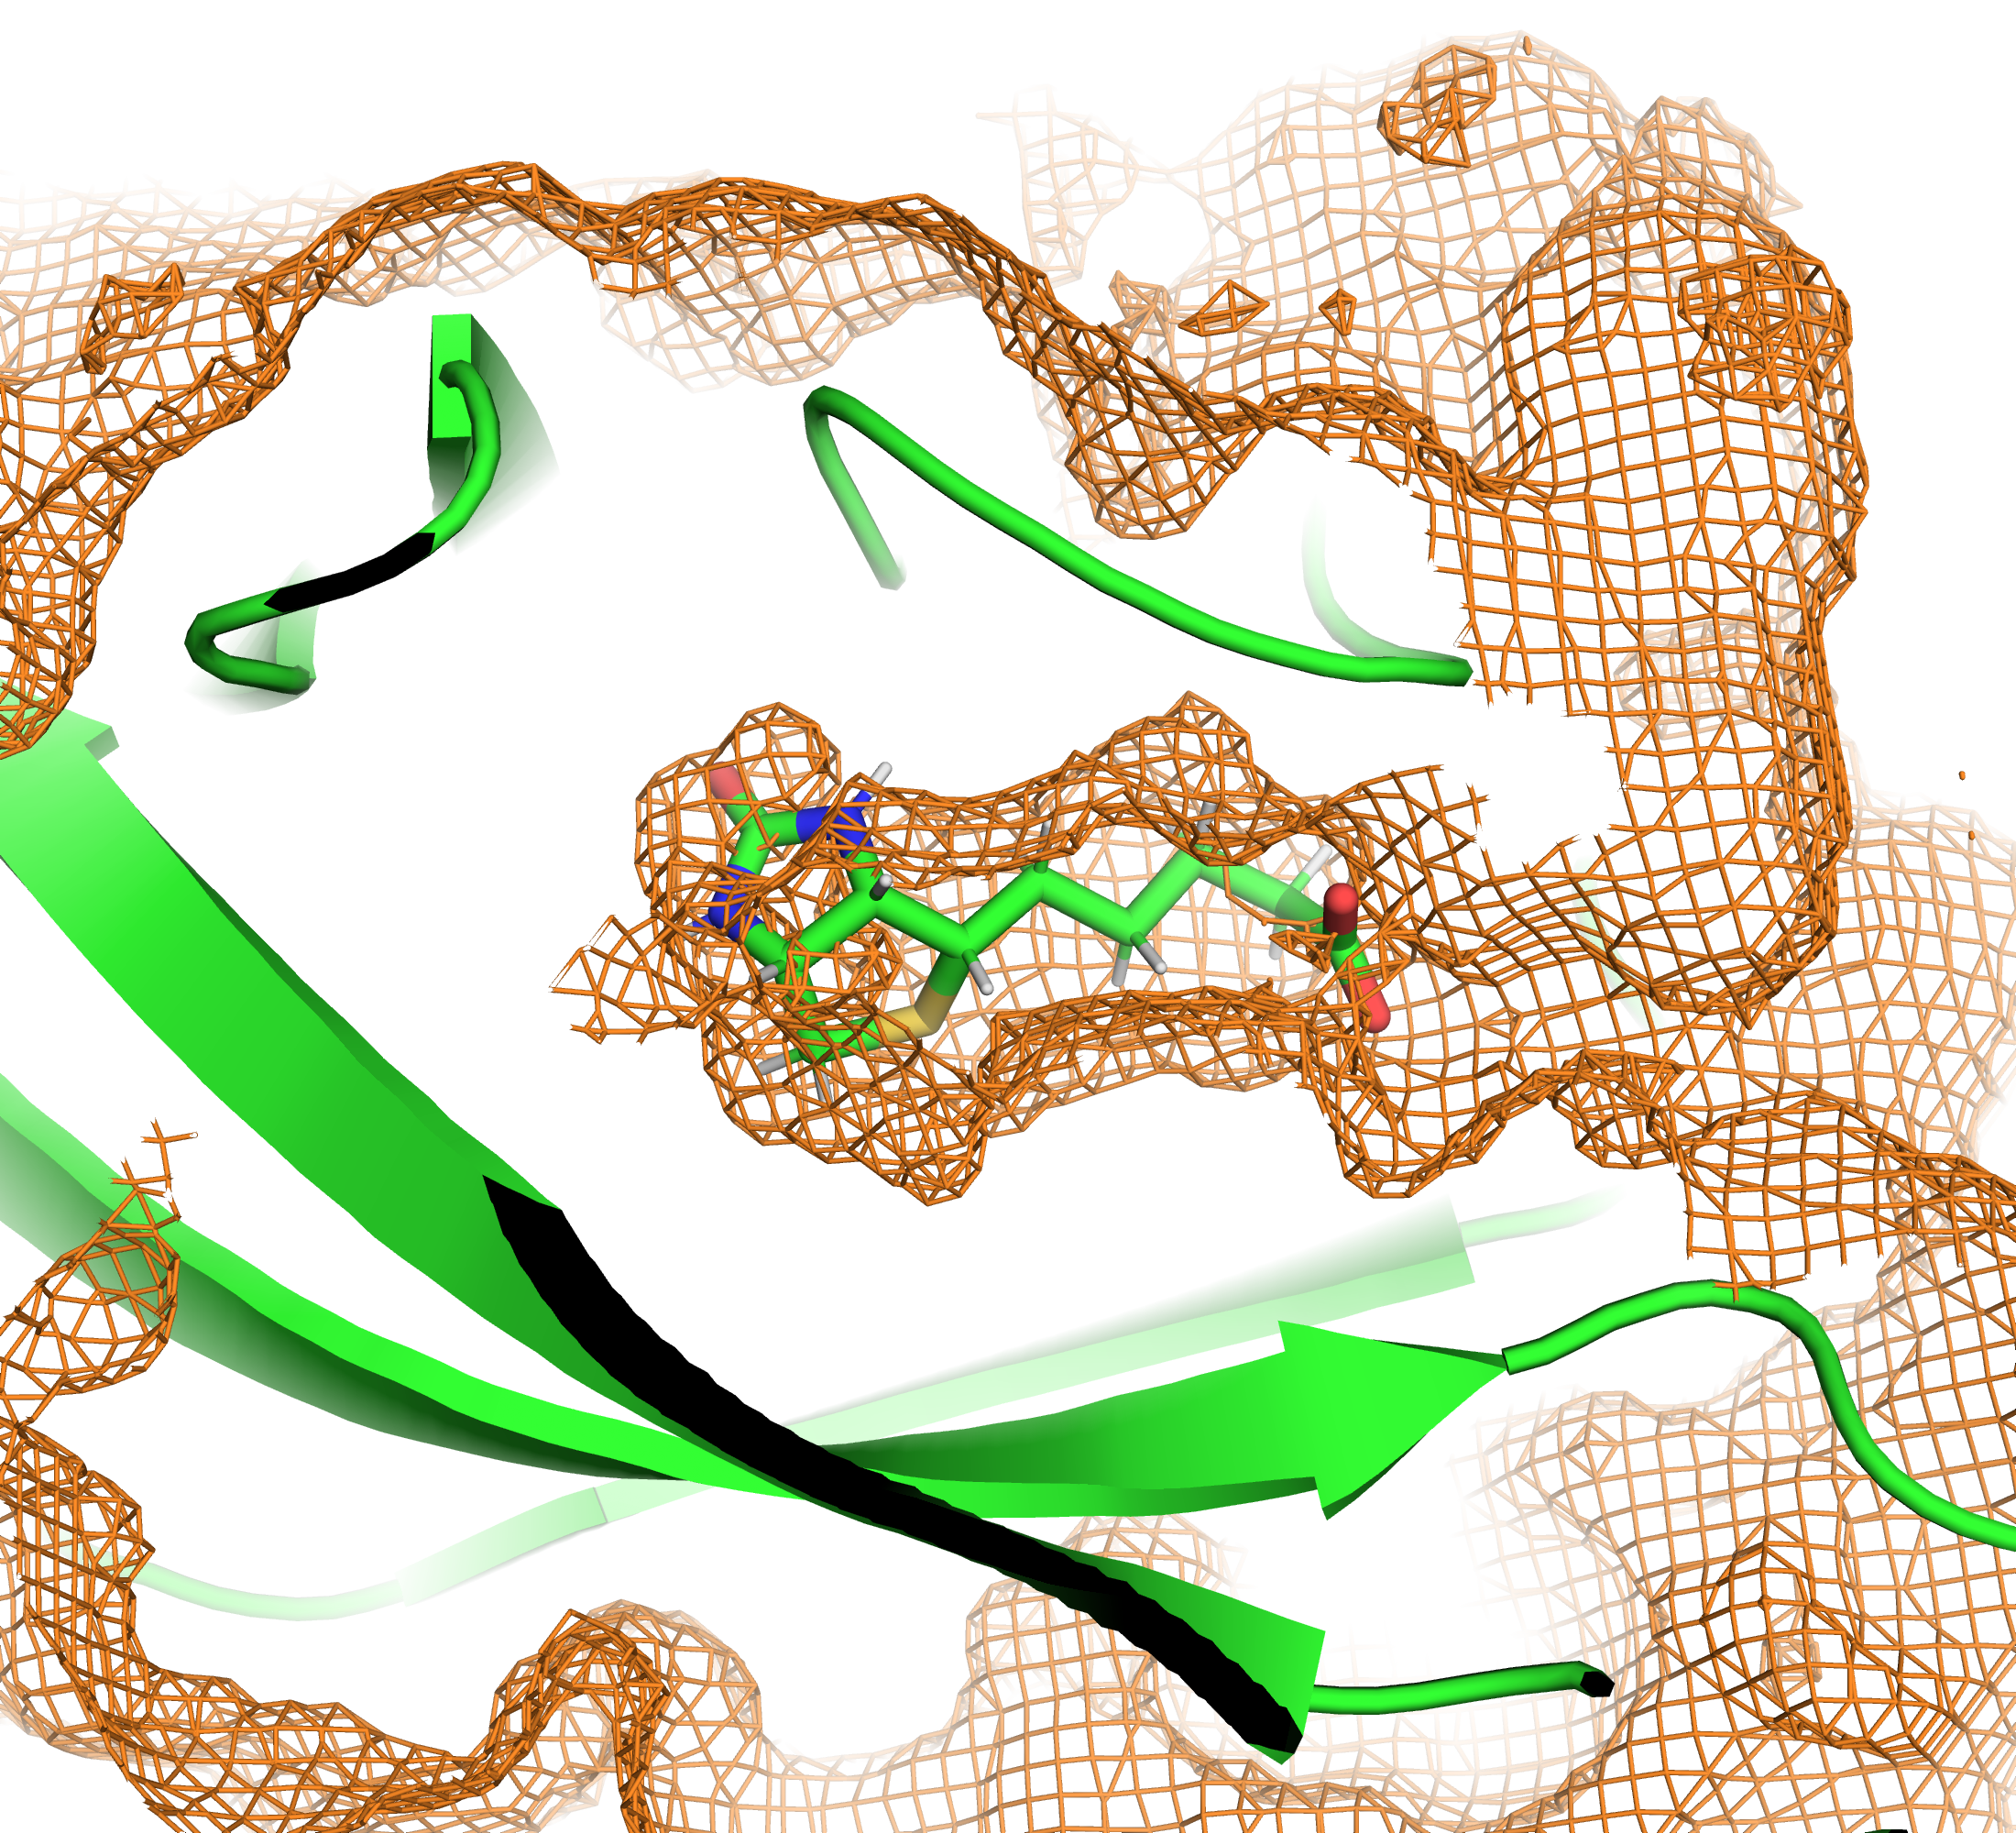
\includegraphics[width=1\linewidth]{figures/sasa-simple.png}
	\caption{SAS for streptavidin focused on the binding pocket}\label{fig-streptavidin_sasa}
\end{figure}
\subsection{Defining the binding pocket}
Specific regions in a protein can be defined to calculate the thermodynamic quantities for that region.
This is significant specially when calculating the properties of water that will be expelled when a ligand binds to the protein.\\
For example, voxels that are located within the binding pocket can be defined using a ligand solute molecule and a distance criteria. 
In section~\ref{sec:binding_contributions}, we show how to integrate over regions such as the binding pocket. To visualize the considered region, we can create a OpenDX file where we set the considered voxels to 1 and all others to 0. Here, we show what this would look like for a radius of \SI{3.5}{\angstrom} around the heavy atoms of biotin. 

\begin{lstlisting}[style=python]
import gisttools as gt
def select(traj, sel):
	""" 
	Slice a Trajectory by selection mask. 
	"""
	return traj.atom_slice(traj.top.select(sel))
### Load GIST data
compl = gt.gist.load_gist_file(
	'complex/gist/gistoutlong.dat', 
	struct='complex/gist/gist_nowat.pdb')
### Define ligand atoms and find voxels around them
rmax = 3.5
biotin_mask = 'resname BTN and not element H'
btn = select(compl.struct, biotin_mask).xyz[0] * 10.
ind, _, _ = compl.distance_to_spheres(btn, rmax)

### Set voxels within 3.5A of biotin to 1, write out dx file
compl.loc[ind, 'BP'] = 1
compl.save_dx('BP', 'binding_pocket.dx')
\end{lstlisting}

\begin{figure}
	\centering
	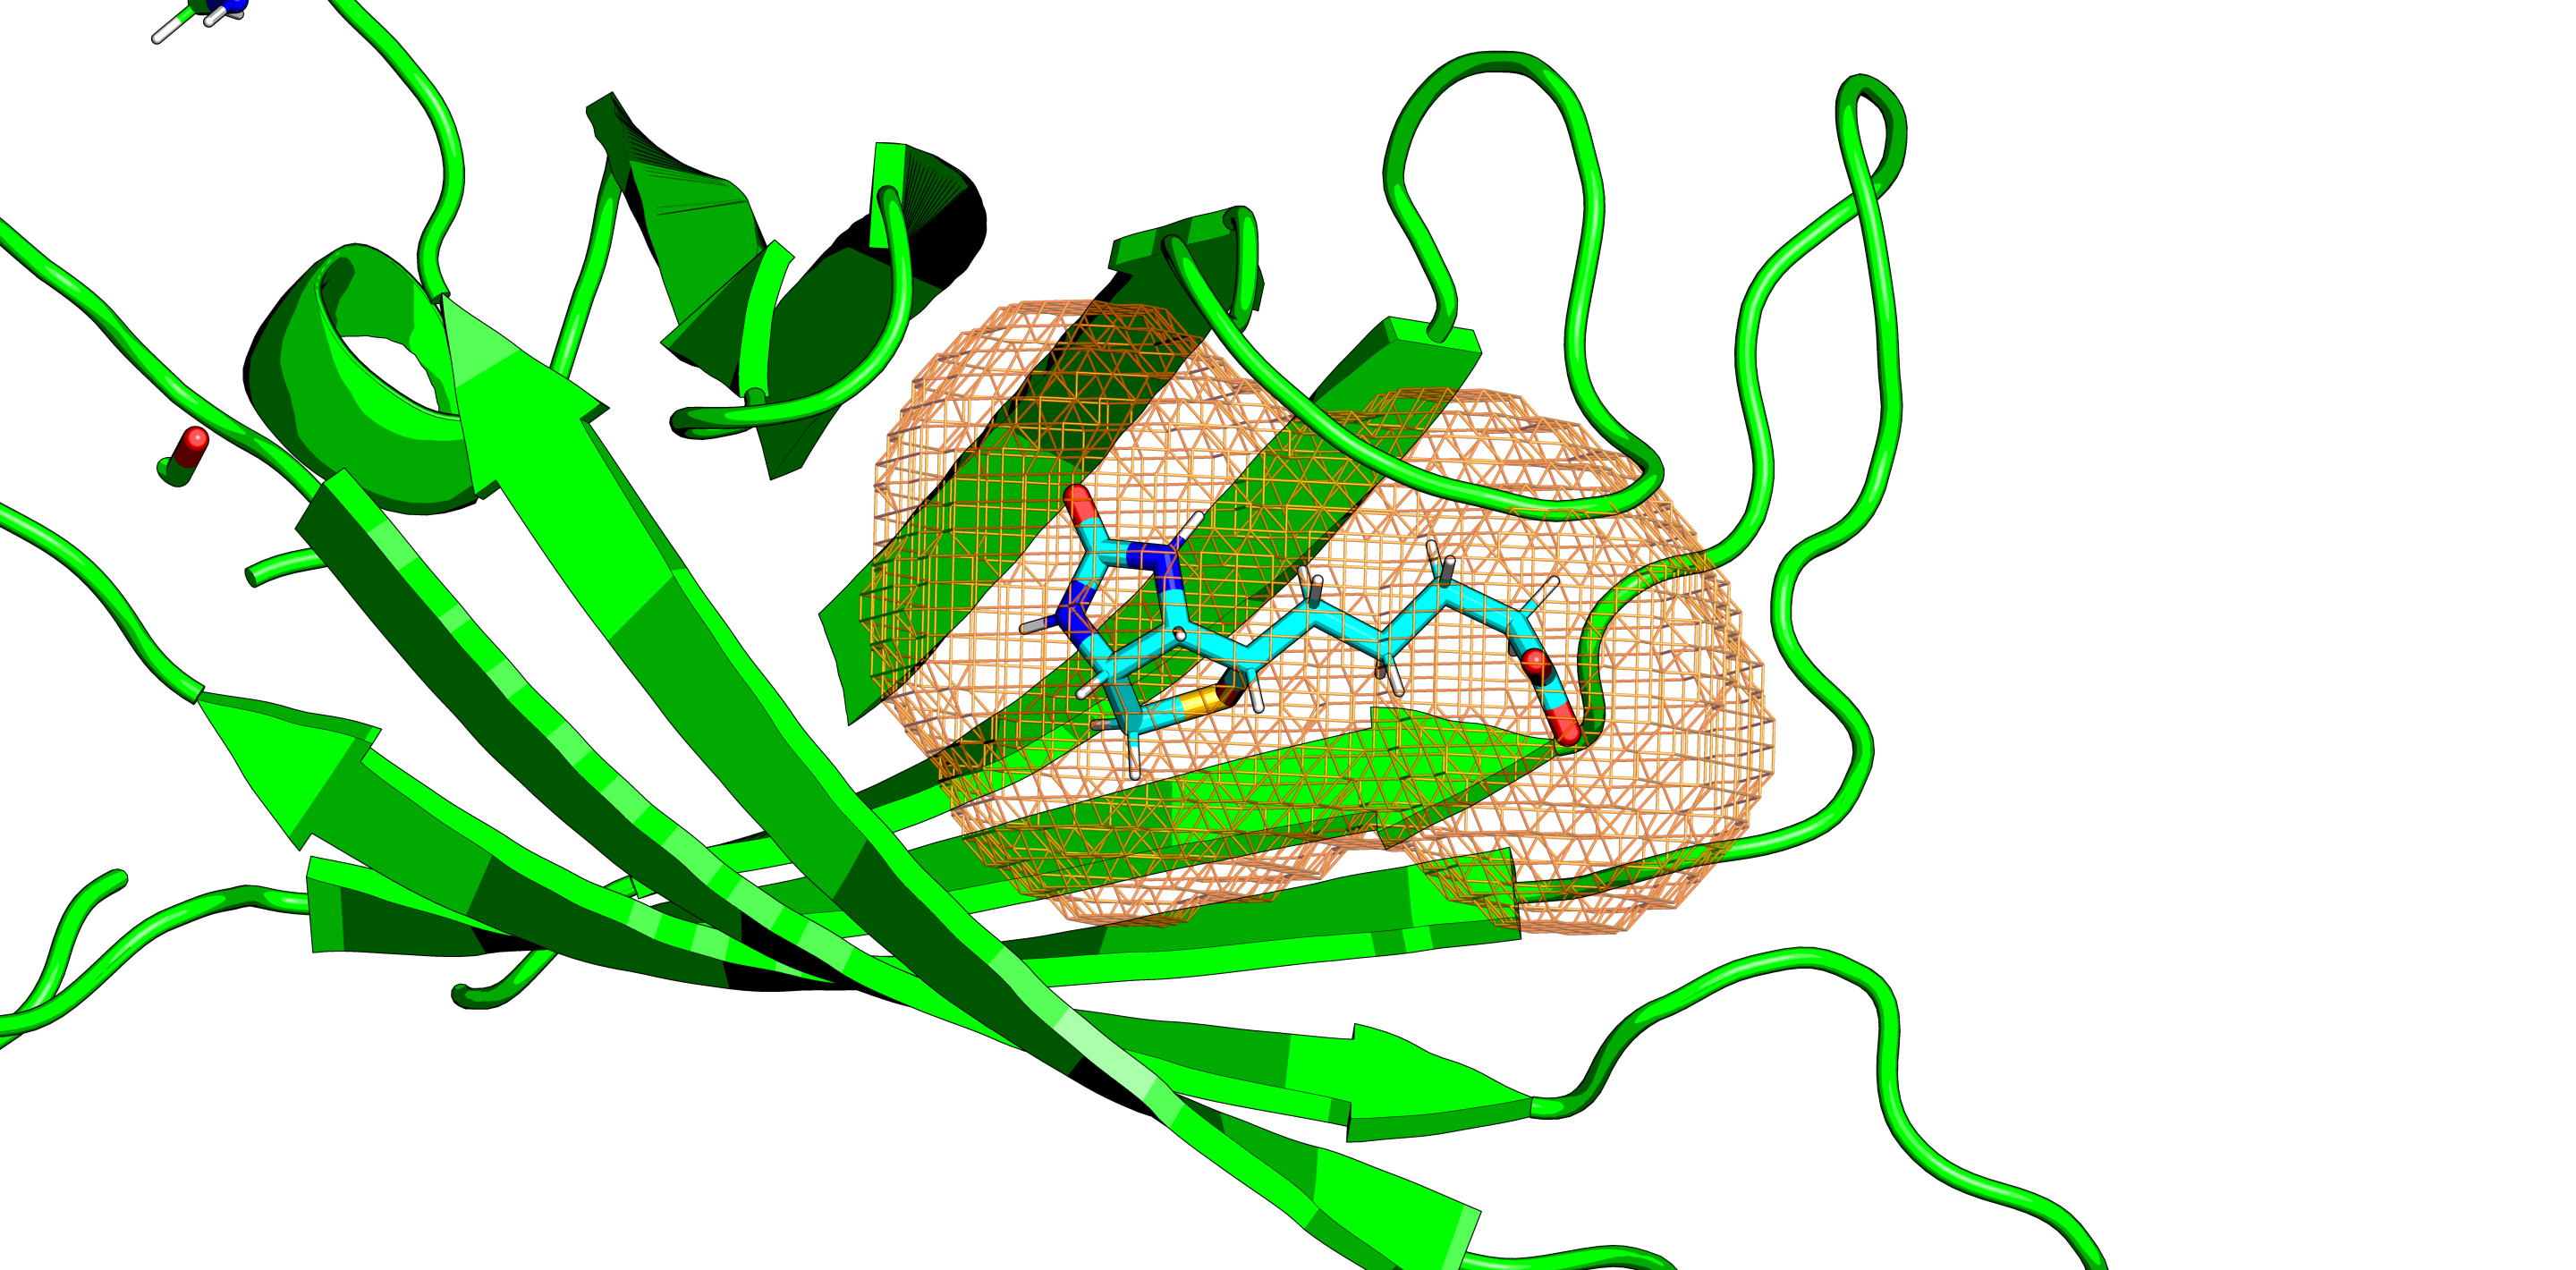
\includegraphics[width=1.0\linewidth]{streptavidin_bp_close.png}
	\caption{Volume of streptavidin defined around \SI{3.5}{\angstrom} of biotin. }\label{streptavidin_volume}
\end{figure}
%TODO: Hide capping group
\pagebreak %TODO pagebreak
\section{Theory}
\label{sec:theory}
GIST is an implementation of inhomogeneous fluid solvation theory (IST) \cite{Lazaridis1998} that discretizes the free energy of solvation $\dgsolv$ on a three-dimensional grid. 
It was first devised by Nguyen et al.\ \cite{Nguyen2012} and its implementation in \software{cpptraj} was thoroughly described by Ramsey et al.\ \cite{Ramsey2016}.
Here, we only provide a short overview of the theory behind GIST.
For more technical information (such as implementation details), we recommend one of the more recent publications on developments in GIST \cite{Kraml2020,Chen2021,Roe2023-mpi-gist}.

\subsection{Solvation Entropy}

%\begin{equation}
%	\Delta S_\textit{solv} = \Delta S_\textit{sw} + \Delta S_\textit{ww}
%\end{equation}
%Here the solvation entropy is approximated from the contribution of solute-water interaction. 
%\textbf{STILLNEEDS REVISON + ADD CITATIONS} The quantity $k_\textit{b}$represents the Boltzman constant, 
%$\rho^\textit{o}$ is the bulk number density, $g_\textit{sw}\left(\textbf{r},\omega \right)$ is the solute-water 
%pair correlation function in the solute's frame of reference, \textbf{r} is the coordinates of the oxygen atom of the water solvent molecule,  
%$\omega$ represents the Euler angles, and $\frac{1}{8\pi^2}$ is the volume of the orientational space, which acts as a normalization constant.
%In bulk and in regions where the orientational 
%entropy is uniform, the quantity $g_\textit{sw}\left(\textbf{r},\omega \right)$ is unity which leads to the first-order solvation entropy of 
%bulk to be zero. Also, this quantity reaches unity as the distance from the solute molecule increases which leads for the calculation of 
%the solvation entropy to be an approximation of the integral around the solute atom. 

IST expresses the free energy of solvation in terms of the solvent density in a coordinate system defined by the solute molecule.
The solute molecule is kept fixed in space, following the standard solvation process established by Ben-Naim \cite{ben-naim-book}.

The entropy can be approximated as an infinite expansion of correlations of increasing order.
In a slightly simplified view, the first order is the log solvent density $ln\left(g_\textit{sw}\left(\textbf{r},\omega \right)\right)$ at each position $\textbf{r}$ and orientation $\omega$.
The first-order entropy omits all solvent-solvent (and higher) correlations, while the solute-solvent correlation is taken into account because the coordinates are relative to the solute.
Thus, it is called the solute-water entropy $S_{sw}$.
%The second order is the pair density, i.e., the probability of finding two solvent molecules in positions $\textbf{r}$ and $\textbf{r}^\prime$.
The solvent density is expressed relative to the bulk density $\rho^0$. %$g_\textit{sw}\left(\textbf{r},\omega \right)$ is the solute-water 
%pair correlation function in the solute's frame of reference, \textbf{r} is the coordinates of the oxygen atom of the water solvent molecule,  
%$\omega$ represents the Euler angles, and 
The entropy integral is also normalized by $8\pi^2$, which is the volume of the orientational space.
In bulk or at a high distance to the solute molecule, the quantity $g_\textit{sw}\left(\textbf{r},\omega \right)$ approaches one, which leads to zero first-order entropy. 
Therefore, no reference entropy is needed unless there is a numeric bias, e.g., when the MD frames are statistically dependent because the time between them is insufficient.
\begin{equation}
	\Delta S_\text{solv}
	\approx \Delta S_\textit{sw}
	\newcommand{\gro}{g_{sw}(\textbf{r},\omega)}
	\equiv -R \frac{\rho^0}{8\pi^\textit{2}} \int \gro \ln\gro d\textbf{r}d\omega
\end{equation}

\subsubsection{Entropy Calculations in cpptraj}
In \software{cpptraj}, the calculation of solvation entropy is handled by two methods.\\
In the first method, the solvation entropy is broken down into translational and orientational contributions.
\begin{equation}
\Delta S_\textit{solv} = \Delta S_\textit{trans} + \Delta S_\textit{orient}
\end{equation}
This is exact assuming that the distribution of the orientation $\omega$ is constant within a voxel $k$, but might converge slower than computing the entropy from the combined space (see below).
The second method directly calculates the solvation entropy by evaluating the six-dimensional integral (3 for position and 3 for orientation).

%\begin{equation}
%g_\textit{vox} \left( \textbf{r}, \omega \right) \approx g_\textit{vox}(\textbf{r}) g_\textit{vox}(\omega)
%\end{equation}
A first nearest neighbor (NN) approach is used to evaluate the entropy based on the orientational and translational distributions.
The distributions are computed relative to a homogeneous distribution of solvent molecules, given a bulk density $\rho^0$.
The average entropy contributions per solvent molecule in voxel $k$ are calculated as

\begin{equation}
	S_{k}^\textit{trans} = -R \left( \gamma + \frac{1}{N_\textit{k}} \sum _{i=1}^{N_k} \ln g_{NN, \textit{i}}(\textbf{r}) \right),
\end{equation}
\begin{equation}
S_{k}^\textit{orient} = -R \left( \gamma + \frac{1}{N_k} \sum _{i=1}^{N_k} \ln g_{NN, i}(\omega) \right)
,
\end{equation}
and
\begin{equation}
S_\textit{k}^\text{six} = -R \left( \gamma + \frac{1}{N_\textit{k}} \sum _{i=1}^{N_k} \ln g_{NN, \textit{i}}(\textbf{r},\omega) \right),
\end{equation}
where $N_\textit{k}$ is the number of water solvent molecules found in voxel k, $\gamma$ is Euler's constant accounting for the bias of the naive entropy estimator, and $g_\textit{NN}$ is the nearest neighbor estimate of the density.

\subsection{Solvation Energy}
The solvation energy is calculated from the water-water and water-solute interactions from the force field.
\begin{equation}
	\Delta E_\textit{solv} = \Delta E_\textit{sw} + \Delta E_\textit{ww}
\end{equation}
The solute-solvent energy $E_{sw}$ can be expressed in terms of the solvent density and the potential $U_{sw}(\textbf{r},\omega)$ induced by the solute molecule.
In practice, $E_{sw}$ is computed as the expectation value $\langle\cdot\rangle$ of the pairwise force field energy $U_{ij}$ between all solvent molecules in voxel $k$ and all solute atoms.

\begin{equation}
	\begin{aligned}
		\label{eq-esw}
		\Delta E_{sw}(\textbf{r}) \equiv& \frac{1}{8\pi^2} \int g_\textit{sw}\left(\omega|\textbf{r}\right) U_\textit{sw}\left(\textbf{r}, \omega\right) d\omega \\
		\Delta E_{sw,k}=& \left\langle \sum_i^{\textit{solvent},k} \; \sum_j^\textit{solute} U_{ij}\right\rangle
	\end{aligned}
\end{equation}
To localize $E_{sw}$ on the three-dimensional grid, every energy term is assigned to the voxel $k$ holding the solvent, and the expectation value in Equation~\ref{eq-esw} is computed per voxel.
Similar to the entropy integrals, the solute-water solvation energy decays with increasing distance to the solute molecule.
Hence, it can be approximated by local spatial integrals. 
The solvent-solvent energy $E_{ww}$ is computed similarly.
It can also be expressed in terms of density functions, but is practically computed as a sum over solvent-solvent interactions per voxel $k$.
In contrast to $E_{sw}$, $E_{ww}$ does not tend to zero in bulk.
Therefore, a reference corresponding to the average energy of a bulk water solvent molecule needs to be subtracted.
The referenced solvent-solvent energy will be denoted as $E_{ww}^\text{corr}$.

\begin{equation}
	\begin{aligned}
		\Delta E_{ww}^\text{corr}(\textbf{r}) \equiv & \left(\frac{1}{8\pi^2} \right)^2 \rho^o \int g_{sw}(\omega|\textbf{r}) \\
			& \times \left[g_{sw}(\textbf{r}^\prime , \omega^\prime) - g^0_{ww} (\textbf{r}, \omega, \textbf{r}^\prime, \omega^\prime )\right] \\
			& \times U_{ww}(\textbf{r}, \omega, \textbf{r}^\prime, \omega^\prime)d\omega d\textbf{r}^\prime d\omega^\prime \\
		\Delta E_{ww,k}^\text{corr} =& \frac{1}{N_k} \left\langle \sum_i^{\text{solvent},k} \; \sum_{j \neq i}^\text{solvent} U_{ij}\right\rangle - \left\langle E_{ww}^\text{bulk}\right\rangle
	\end{aligned}
\end{equation}

\subsubsection{Interpreting the energy values}
When computing the total $E_{ww}$ of the system, double-counting of interactions must be avoided.
The total solvent-solvent energy of the system is as follows:

\begin{equation}
	\Delta E^\text{R}_{ww} = \sum_{k}^\text{voxels} \frac{E_{ww,k}^\text{corr}}{2}
%	\Delta E^R_{ww} = n^R E^\text{bulk}_{ww} - E^\textit{R,corr}_{ww}
\end{equation}
However, when water is replaced from a small region $R$ of interest, such as a single water solvent molecule, almost all interactions are with water solvent molecules outside of this region.
Therefore, there is no double counting, and the full solvent-solvent energy should be used.

\begin{equation}
	\Delta E^\text{R}_{ww} = \sum_{k}^{\text{voxels in }R} E_{ww,k}^\text{corr}
%	\Delta E^\textit{R,norm}_\textit{ww} = E^\textit{R,norm}_\textit{ww} - 2E^\textit{bulk}_\textit{ww}
\end{equation}
When the region $R$ comprises more than one solvent molecule, interactions within this region are double-counted while interactions to the outside are not.
This could be solved using the solvent-solvent energy between each pair of voxels $E_{ww,k\;l}$:
\begin{equation}
	\Delta E^\text{R}_{ww} = 2\left(\sum_{k}^\text{voxels in R} E_{ww,k}^\text{corr}-\sum_{k}^\text{voxels in R}\sum_{l}^\text{l>k} E_{ww, k\;l}\right)
\end{equation}
While this is supported by the standard GIST implementation (using the \inlinecode{doeij} flag), it is rarely done due to the large size of the $E_{ww,k\;l}$ matrix.
Integrating GIST values over the whole grid corresponds to a process where all the solvent is removed into bulk.
However, when integrating over a small region, this process is less well-defined, since it is unclear to what extent the remaining solvent would reorganize.
This depends on the local environment and on \emph{what} the solvent would be replaced by.
Therefore, the effect of reorganization must be judged for each case individually.
One way to treat reorganization is an end-state approach as shown in the tutorial: all states before and after solvent reorganization are considered. In the tutorial, this corresponds to the solvation of biotin and streptavidin seperated (initial states) and in complex (end-state). Note that all solvent contributions need to be considered to get thermodynamically accurate results in such a case. In practice this therefore requires the integration over the whole grid or at least all voxels with solvent properties different from bulk (i.e. setting a large cutoff).
\subsubsection{PME energy}
In the original version of GIST, the energies are calculated based on the the minimum image convention.
In PME-GIST, the electrostatic energy $E_\text{elec}$ is calculated using the particle mesh Ewald (PME) method, which yields energies that are highly consistent with the Amber MD engine \cite{Chen2021}.
The Lennard-Jones part $E_\text{lj}$ is computed separately in direct space.

\begin{equation}
	E_\text{total} = E_\text{elec} + E_\text{lj}
\end{equation}
During the electrostatics calculation, the system is treated as periodic and the energy is split into a short-range term $E_\text{dir}$, which is calculated in direct space using a distance cutoff, and a long-range term $E_\text{rec}$, which is calculated in reciprocal space.
Additionally, there is a correction term $E_\text{self}$ (called $E_\text{corr}$ in the original publication \cite{Chen2021}), which corrects for the self-interaction of each solvent molecule in the reciprocal term.
\begin{equation}
	E_\textit{elec} = E_\text{dir} + E_\text{rec} + E_\text{self}
\end{equation}
The short-range Lennard-Jones contribution is computed in the direct space using a distance cutoff.
Furthermore, a long-range correction term is computed that accounts for the contributions above this cutoff assuming a homogeneous distribution of particles.

\begin{equation}
	E_\text{lj} = E_\text{lj,\ short} +  E_\text{lj,\ corr}
\end{equation}

\section{Checklists and Cheat Sheats} \label{sec:checklists}
%Tutorials do not necessarily require the use of a checklist as in Best Practices documents; however, they can include these if desired.
%Several useful checklist formats are available, with examples presented in \texttt{sample-document.tex} in \url{github.com/livecomsjournal/article_templates/templates}.
%One example is shown here.

% Here is a single-column checklist that consists of multiple sub-checklists
\begin{Checklists}[H]
	
	\begin{checklist}{Simulation settings}
		\textbf{Each number denotes the minimum setting, with the optimum in brackets.}
		\begin{itemize}
			\item Simulation time: \SIrange{10}{20}{\nano\second} (\SI{100}{\nano\second})
			\item Number of analyzed frames: \num{10000} (\num{100000})
			\item Restraints: typically \SI{100}{\kcalPerMolASqr} on solute heavy atoms. Minimum: \SI{10}{\kcalPerMolASqr}
		\end{itemize}
	\end{checklist}
	
	\begin{checklist}{Choosing an energy method}
		\begin{itemize}
			\item CPU: slow, most general (can write out $E_{ij}$ matrices)
			\item CPU, PME: highly consistent with Amber MD, fast
			\item GPU, direct space: fastest for a single CPU core
		\end{itemize}
	   
	All methods profit from MPI-parallelization.   
	PME with multiple CPU cores (>4) is usually the fastest method.
	\end{checklist}
	
	\begin{checklist}{Obtaining absolute $\Delta G_\textup{solv}$}
		\begin{itemize}
			\item Check the radial convergence (see Fig.~\ref{fig_radial_convergence})
			\item Choose a sufficient distance cutoff
			\item Choose an optimal $E_{ww}$ reference value
			\item Tweak simulation length and number of frames to obtain smooth free energy contributions and unbiased (i.e., zero) bulk entropy.
			\item If necessary, subtract an entropy reference
		\end{itemize}
	\end{checklist}
	
	\begin{checklist}{Handling convergence problems}
		\begin{itemize}
			\item Insufficient sampling leads to high noise in the results. Use higher numbers of frames.
			\item Correlation between frames leads to negative entropy in bulk. Increase simulation time and/or reduce the number of frames.
		\end{itemize}
	\end{checklist}
	
	%\begin{checklist}{A list}
	%\textbf{Single-column checklists are also straightforward by removing the asterisk}
	%\begin{itemize}
	%\item First thing let's do an item which breaks across lines to see how that looks
	%\item Also remember
	%\item And finally
	%\end{itemize}
	%\end{checklist}
	%
	%\begin{checklist}{Another list}
	%\textbf{This is some further description.}
	%\begin{itemize}
	%\item First thing
	%\item Also remember
	%\item And finally
	%\end{itemize}
	%\end{checklist}
	
\end{Checklists}
%\section{Cheat sheet}
%This will be a cheatsheet containing all options for cpptrajs GIST implementation
%The checklist ``The CPPTRAJ GIST action'' provides a cheat sheet summarizing the important options to the GIST action and its output, as well as frequently used equations.

%\subsection{Installation}
%GIST calculations in cpptraj can be sped up through various levels of 
%parallelization.
%If cpptraj was compiled with the '-cuda' configure flag set, the GPU accelerated version of GIST is used automatically. 
%In addition, OpenMP and MPI parallelization are available if cpptraj was compiled the necessary options. 
%
%For detailed instructions on how to install \software{cpptraj}, we refer the reader to the AmberMD GitHub page \url{https://github.com/Amber-MD/cpptraj}.
\FloatBarrier
\begin{Checklists*}[h!]
\begin{checklist}{The CPPTRAJ GIST action}\label{cheatsheet}

\textbf{Options}\\
Various flags and options can be provided when running a GIST calculation in cpptraj. 
A list of possible and required options is provided here:
\medskip

\begin{tabularx}{\textwidth}{@{}l X @{} }
\toprule
\textbf{I/O Options} &\\
name <dataset name> & Name for output datasets in cpptraj. \\
prefix <prefix> & Output file name prefix. Default is 'gist'.\\
ext <extension> & Output grid file name extension. Default is  '.dx'. \\
out <file> & Name of the main GIST output file. If not specified set to '<prefix>-output.dat'.\\
info <file> & Name of main GIST info file. If not specified info is written to standard output. \\
floatfmt <fmt> & Format for floating point values in GIST output file. Options are 'double', 'scientific' or 'general'. Default chooses 'fixed' or 'scientific' automatically. \\
floatwidth <val>& Width of floating point values in GIST output file. Default is no width restriction. \\
floatprec <val>& Precision of floating point values in GIST output file. Default is the system default. \\
intwidth <val>& Width of integer point values in GIST output file. Default is no width restriction. \\
doeij & Output the triangular matrix representing the water-water 
interactions between pairs of voxels. Not supported with PME or GPU GIST.\\

\textbf{Grid Options} &\\
gridcntr <xval> <yval> <zval> & Coordinates in \AA{} of the center of the grid. Default is 0.0, 0.0, 0.0. \\
griddim <xval> <yval> <zval> & Grid dimensions in voxels along each coordinate axis. Default is 40, 40, 40.\\
gridspacn <val> & Grid spacing (linear dimension of each voxel) in 
Angstroms. Default is \SI{0.5}{\angstrom}.\\
rmsfit <mask> & If specified, grid will be rotated and translated to follow the atoms selected by mask. \\
\textbf{GIST Calculation Options} &\\

skipE & Skip all the energy calculations (cannot be specified with ’doeij’)\\
skipS & Skip all the entropy calculations.\\
refdens <val> & Reference density of bulk solvent, used in computing 
$g_O, g_H$, and the translational entropy. Default is 0.0334 molecules/\si{\cubic\angstrom}. \\
temp <val> & Temperature of the input trajectory. \\
noimage &  Disable distance imaging in energy calculation. \\

neighborcut <val> & Cutoff in \si{\angstrom} for determining solvent O-O neighbors. Default is \SI{3.5}{\angstrom}. \\

oldnnvolume & Use the old reference volume for the nearest neighbor entropy. \\

nnsearchlayers <val> & Layers of neighboring voxels considered in nearest neighbor search. Higher values may improve entropy convergence for little sampling or fine grid spacings, but increase the calculation time. Default is 1. \\

\textbf{PME Options} & \\
nopme & Do not use particle mesh Ewald for the non-bonded calculation. This is set  on default. \\
pme & Use particle mesh Ewald for the non-bonded electrostatics calculation. The van der Waals energy will be calculated using a long-range correction for periodicity.\\
\qquad cut <val> & Direct space cutoff for pme. Default is \SI{3.5}{\angstrom}.\\
\qquad dsumtol <val> & Direct sum tolerance used to determine Ewald coefficient. Default is 0.00001.\\
\qquad ewcoeff <val> & Ewald coefficient in 1/Å. \\
\qquad erfcdx <val> & Spacing to use for the ERFC splines. Default is \SI{0.0002}{\angstrom}. \\
\qquad skinnb & Used to determine pairlist atoms (added to cut, so pairlist cutoff is cut + skinnb); included in order to maintain consistency with results from sander. \\
\qquad ljswidth <val> & If specified, use a force-switching form for the Lennard-Jones calculation from <cutoff>-<val> to <cutoff> \\
\qquad order <val> & Spline order for charges. \\
\qquad nfft <nfft1>,<nfft2>,<nfft3> & Explicitly set the
number of FFT grid points in each dimension.
Will be determined automatically if not
specified. \\

\end{tabularx}  
\end{checklist}
\end{Checklists*}
\begin{Checklists*}[h!]
\begin{checklist}{The CPPTRAJ GIST action}
	
\textbf{Further Options}\\
\begin{tabularx}{\textwidth}{@{} l X @{}}
\toprule

\textbf{Solvent Options} &\\
solute <mask> & Selection mask for the solute. All other molecules will be solvent. If this is omitted, the standard solute/solvent assignment will be used. \\
solventmols <mols> &Comma-separated list of solvent molecules residue names. Energies will be computed per solvent molecule. For the entropy, only the first solvent will be used. Use this for calulations with more than one solvent of interest, e.g. for  ions. \\
rigidatoms <c> <a1> <a2> & Specifies the molecular orientation for the entropy calculation from a central atom and two additional atoms, e.g. O H1 H2 for water. By default, a simple heuristic will be used.  
Use this option if the automatically chosen atoms are collinear or do not represent the orientation well. \\
nocom & Do not use the center of mass to define the molecular position. Instead, use the first atom in rigidatoms. Use this flag to restore the behavior of old GIST runs. \\
\textbf{Order Calculation Options} &\\
doorder & Calculate the water order parameter [reference] for each voxel\\
\qquad nopl & Do not use pair list for order calculation\\
\qquad plcut <val> & Pair list cutoff for order calculation. Default is \SI{10}{\angstrom}\\
\bottomrule
\end{tabularx}   
\medskip


\textbf{Output}\\
GIST calculations write a variety of data sorted by voxel into an outputfile specified by the 'out' keyword. 
Some of the output data is also automatically written to 'open data explorer' (.dx) files for convenient visualisation in software such as VMD or PyMOL. Note that some columns will be written out both with '\_norm' and '\_dens' suffixes, refereing to normalization by solvent molecule or voxel volume respectively.
The following columns can be found in the output file:
\medskip


\begin{tabularx}{\textwidth}{@{}l l X@{}}
\toprule
Name & Keyword & Description\\
\midrule
index & & Voxel indices \\
x, y, z & & Coordinates of the voxel centers \\
pop & & Population of solvent in voxel over entire simulation \\
gX &  & For every element in the main solvent, the number density of atoms found in the voxel, in units of the bulk density. If the same element occurs multiple times, the bulk density is scaled accordingly. \\
g\_mol\_Y & [solventmols]  & Density of every solvent species Y. Scaled by rho0. \\
Esw &  &  Mean solute-solvent interaction energy. \\
Eww &  & Mean solvent-solvent interaction energy. \\
Esw\_mol\_Y & [solventmols]  &  Mean solute-solvent interaction energy for solvent species Y. \\
Eww\_mol\_Y & [solventmols]  & Mean solvent-solvent interaction energy for solvent species Y. \\
PME & [pme] & Solvent PME energy. \\
U\_PME & [pme] & Solvent PME energy. \\
dTStrans &  & First order translational entropy. \\
dTSorient &  & First order orientational entropy. \\
order &  & (if \inlinecode{doorder} was specified) Average Tetrahedral Order Parameter. \\
dipolex &  & x-component of the mean solvent dipole moment density \\
dipoley &  & y-component of the mean solvent dipole moment density \\
dipolez &  & z-component of the mean solvent dipole moment density \\
dipole &  & Magnitude of mean dipole moment density (polarization). \\
neighbor &  & Mean number of solvent molecules neighboring the solvent molecules found in this voxel. \\
order & & Average tetrahedral order parameter \\

\end{tabularx}
\end{checklist}
\end{Checklists*}
\FloatBarrier
\section*{Author Contributions}

%%%%%%%%%%%%%%%%
% This section mustt describe the actual contributions of
% author. Since this is an electronic-only journal, there is
% no length limit when you describe the authors' contributions,
% so we recommend describing what they actually did rather than
% simply categorizing them in a small number of
% predefined roles as might be done in other journals.
%
% See the policies ``Policies on Authorship'' section of https://livecoms.github.io
% for more information on deciding on authorship and author order.
%%%%%%%%%%%%%%%%
All authors were involved in reviewing and editing the original manuscript. \\  
VJH and FW conceptualized the research and co-wrote the initial draft.\\
VM contributed the original drafts of sections \ref{sec:theory} and \ref{sec:visualization}.\\
HC helped with code curation and validation.\\
MLFQ helped with conceptualization and gave writing input for the initial draft. \\
SR and DR contributed technical input.\\  
KRL, MKG and TK were involved with conceptualization, funding acquisition, project management and supervision.\\

% We suggest you preserve this comment:
For a more detailed description of author contributions,
see the GitHub issue tracking and changelog at \githubrepository.

\section*{Potentially Conflicting Interests}
%%%%%%%j
%Declare any potentially competing interests, financial or otherwise
%%%%%%%

MKG has an equity interest in and is a cofounder and scientific advisor of 
VeraChem LLC.

\section*{Funding Information}
%%%%%%%
% Authors should acknowledge funding sources here. Reference specific grants.
%%%%%%%

\section*{Author Information}
\makeorcid

\bibliography{bibliography}

%%%%%%%%%%%%%%%%%%%%%%%%%%%%%%%%%%%%%%%%%%%%%%%%%%%%%%%%%%%%
%%% APPENDICES
%%%%%%%%%%%%%%%%%%%%%%%%%%%%%%%%%%%%%%%%%%%%%%%%%%%%%%%%%%%%

%\appendix


\end{document}
